\mysection{Приложения на обобщените мрежи и симулатора \textit{OnlineGN}}
\hspace*{2.5em}В настоящата глава се разглеждат четири нови ОМ модела на процеси, които до този момент не са били описвани чрез апарата на ОМ. Всеки от разработените модели е симулиран и верифициран чрез програмната среда \textit{OnlineGN}. Изложението и проведените симулации в тези четири раздела представляват решението на \ref{task:new-models} и \ref{task:simulation}. Тези и други разработени модели са публикувани и достъпни в папка \texttt{examples} на хранилището на приложението \cite{phdThesisOnlineGNRepo}.
\subsection{Симулация на крайни автомати чрез обобщени мрежи}

\hspace*{2.5em}В тази глава се показва как краен автомат може да бъде описан и симулиран с помощта на ОМ. Стъпка по стъпка ще се изгради връзката между състоянията и преходите на автомата и съответните елементи на ОМ, така че да е ясно как моделът се превръща в работеща схема. Разгледан е и конкретен пример на краен автомат, за който се изгражда съответната ОМ и се реална симулация с \textit{OnlineGN}. 
При разработването и анализа ще бъде следван подходът, предложен в \cite{DimitrievAutomata}.
В \cite{Atanassov1985GNFA} вече е разгледан начин за представяне на автомати чрез ОМ, но основният акцент е поставен върху теоретичното доказателство за съществуването на такова представяне. Липсва обаче конструкция, която да е директно приложима за симулация в софтуерни среди за ОМ, където биха били нужни конкретни структурни ограничения и оптимизации.

\subsubsection{Основни понятия за крайни автомати}

\paragraph*{Крайни азбуки и езици.}
\mbox{}\\
\emph{Крайна азбука} е крайно множество от символи, обикновено означаван със $\Sigma$. \emph{Низ} (или \emph{дума}) над $\Sigma$ е крайна последователност от символи от $\Sigma$. Празният низ (който не съдържа символи) се обозначава с $\varepsilon$. \emph{Език} $L$ над $\Sigma$ е произволно множество от низове над $\Sigma$, т.е. $L \subseteq \Sigma^*$ (като $\Sigma^*$ е множеството от всички низове със символи от $\Sigma$).
\paragraph*{Детерминиран краен автомат (ДКА).}
\mbox{}\\
\label{def:DFA}
\emph{Детерминираният краен автомат} (ДКА) е петорка \cite{HopcroftMotwaniUllman,Kozen}
\[
\mathcal{A} = (Q,\, \Sigma,\, \delta,\, q_{\textit{start}},\, F),
\]
където:
\begin{itemize}
  \item $Q$ е крайно множество от \emph{състояния};
  \item $\Sigma$ е крайна \emph{азбука};
  \item $\delta : Q \times \Sigma \to Q$ е \emph{функцията на прехода}, която е тотална (т.е.\ дефинирана за всяка двойка $(q,a)$ с $q \in Q$ и $a \in \Sigma$);
  \item $q_{\textit{start}} \in Q$ е \emph{началното състояние};
  \item $F \subseteq Q$ е множеството от \emph{приемащи} (или \emph{крайни}) състояния.
\end{itemize}

На \textbf{Фигура~\ref{fig:dfa_figure}} е илюстриран пример за детерминиран краен автомат.
\begin{figure}[H]
\centering
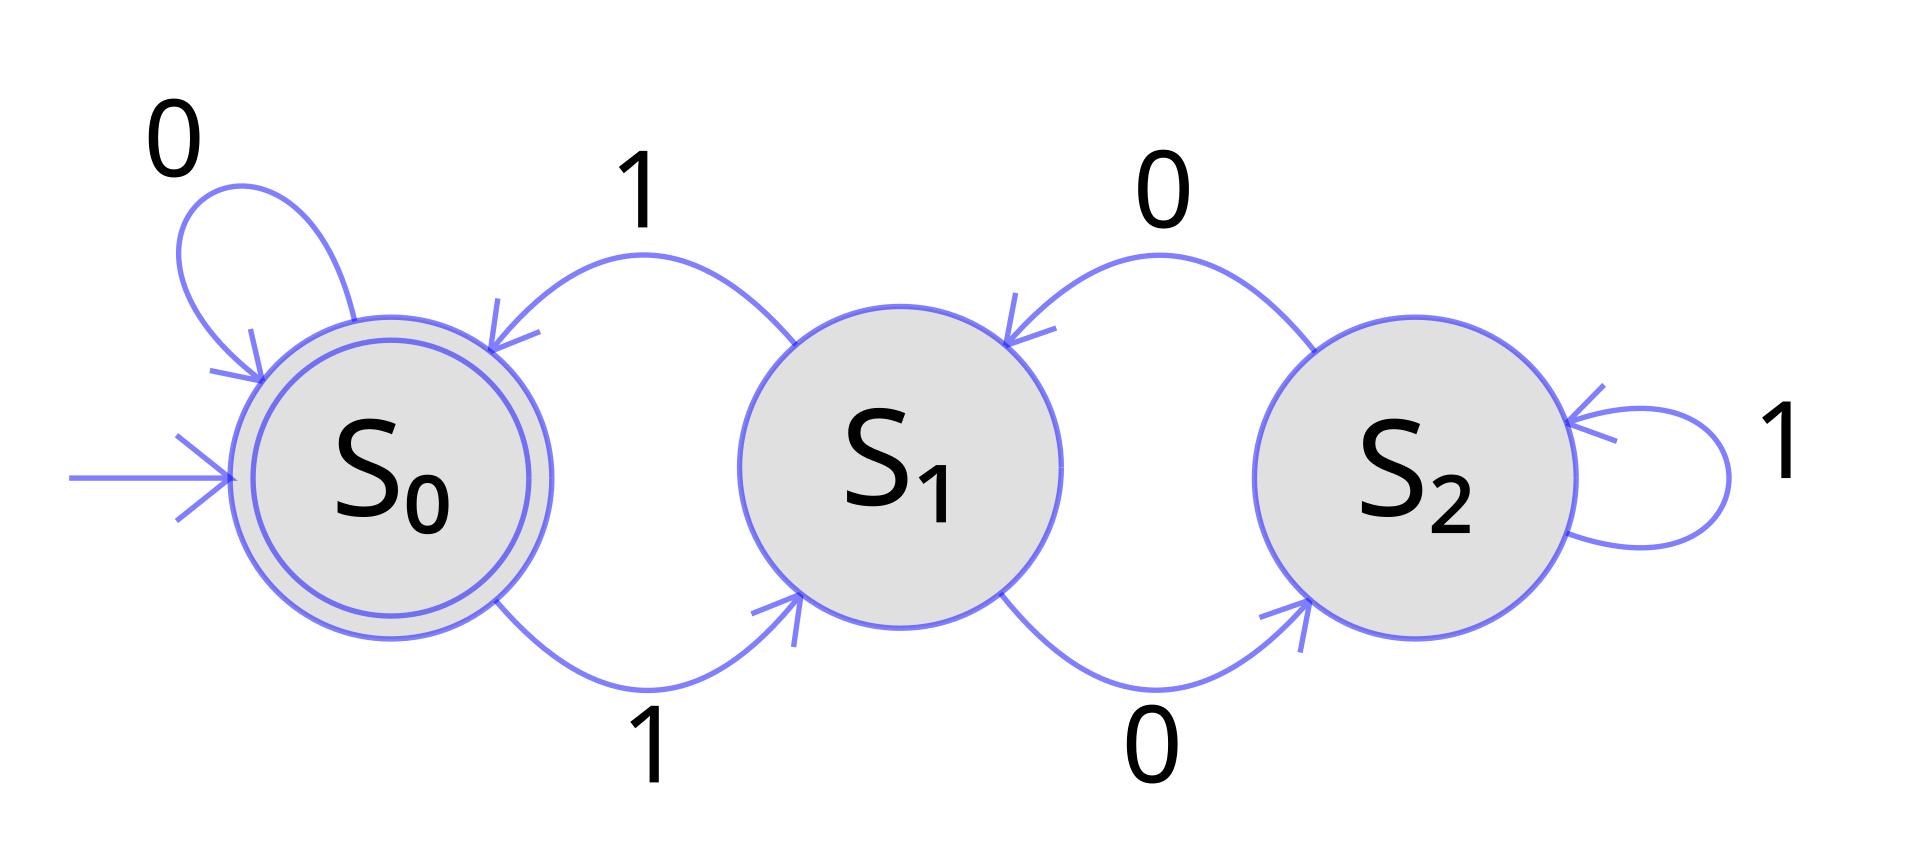
\includegraphics[width=0.6\textwidth]{4. applications/finateStateAutomationsGenNets/images/DFA.png}
\caption{Пример за детерминиран краен автомат.}
\label{fig:dfa_figure}
\end{figure}

\paragraph{Кога ДКА приема дума?}
\mbox{}\\
Нека $\alpha = a_0 a_1 \cdots a_{n-1}$ е дума над азбуката $\Sigma$. ДКА $\mathcal{A}$ \emph{приема} (или \emph{разпознава}) $\alpha$, ако съществува последователност от състояния 
\(
q_0, q_1, \dots, q_n \in Q,
\)
такава че:

\begin{itemize}
	\item началното състояние е $q_0 = q_{\textit{start}}$,
	\item за всяко $0 \le i < n$ преходът е $\delta(q_i, a_i) = q_{i+1}$,
	\item крайното състояние е $q_n \in F$.
\end{itemize}

Еквивалентно, можем да използваме разширената преходна функция \\
\(
\delta^* : Q \times \Sigma^* \to Q
\), която се дефинира индуктивно (виж формула~\eqref{eq:delta-star}):

\begin{equation}
	\delta^*(q, \varepsilon) = q, 
	\quad
	\delta^*(q, \alpha a) = \delta\bigl(\delta^*(q, \alpha), a\bigr),
	\label{eq:delta-star}
\end{equation}
\noindent
където $\varepsilon$ е празната дума.  

Следователно, ДКА $\mathcal{A}$ приема думата $\alpha$ точно тогава, когато
\[
\delta^*(q_{\textit{start}}, \alpha) \in F.
\]


\paragraph{Език на ДКА.}
\mbox{}\\
\emph{Езикът, разпознат} от ДКА $\mathcal{A}$, е 
\[
L(\mathcal{A}) \;=\; \{\,\alpha \in \Sigma^* \,\mid\, \text{$\mathcal{A}$ приема $\alpha$}\}.
\]

\paragraph*{Недетерминиран краен автомат (НКА).}
\label{def:NFA}
\mbox{}\\
\emph{Недетерминираният краен автомат} (НКА) е петорка \cite{HopcroftMotwaniUllman,Papadimitriou}
\[
\mathcal{N} = (Q,\, \Sigma,\, \Delta,\, q_{\textit{start}},\, F),
\]
където:
\begin{itemize}
  \item $Q$ е крайно множество от \emph{състояния};
  \item $\Sigma$ е крайна \emph{азбука};
  \item $\Delta : Q \times \Sigma \to \mathcal{P}(Q)$ е \emph{функцията на прехода}, която за всяка двойка състояние–символ връща \emph{множество от възможни следващи състояния};
  \item $q_{\textit{start}} \in Q$ е \emph{началното състояние};
  \item $F \subseteq Q$ е множеството от \emph{приемащи} (или \emph{крайни}) състояния.
\end{itemize}

На \textbf{Фигура~\ref{fig:nfa_figure}} е илюстриран пример за недетерминиран краен автомат.
\begin{figure}[h!]
\centering
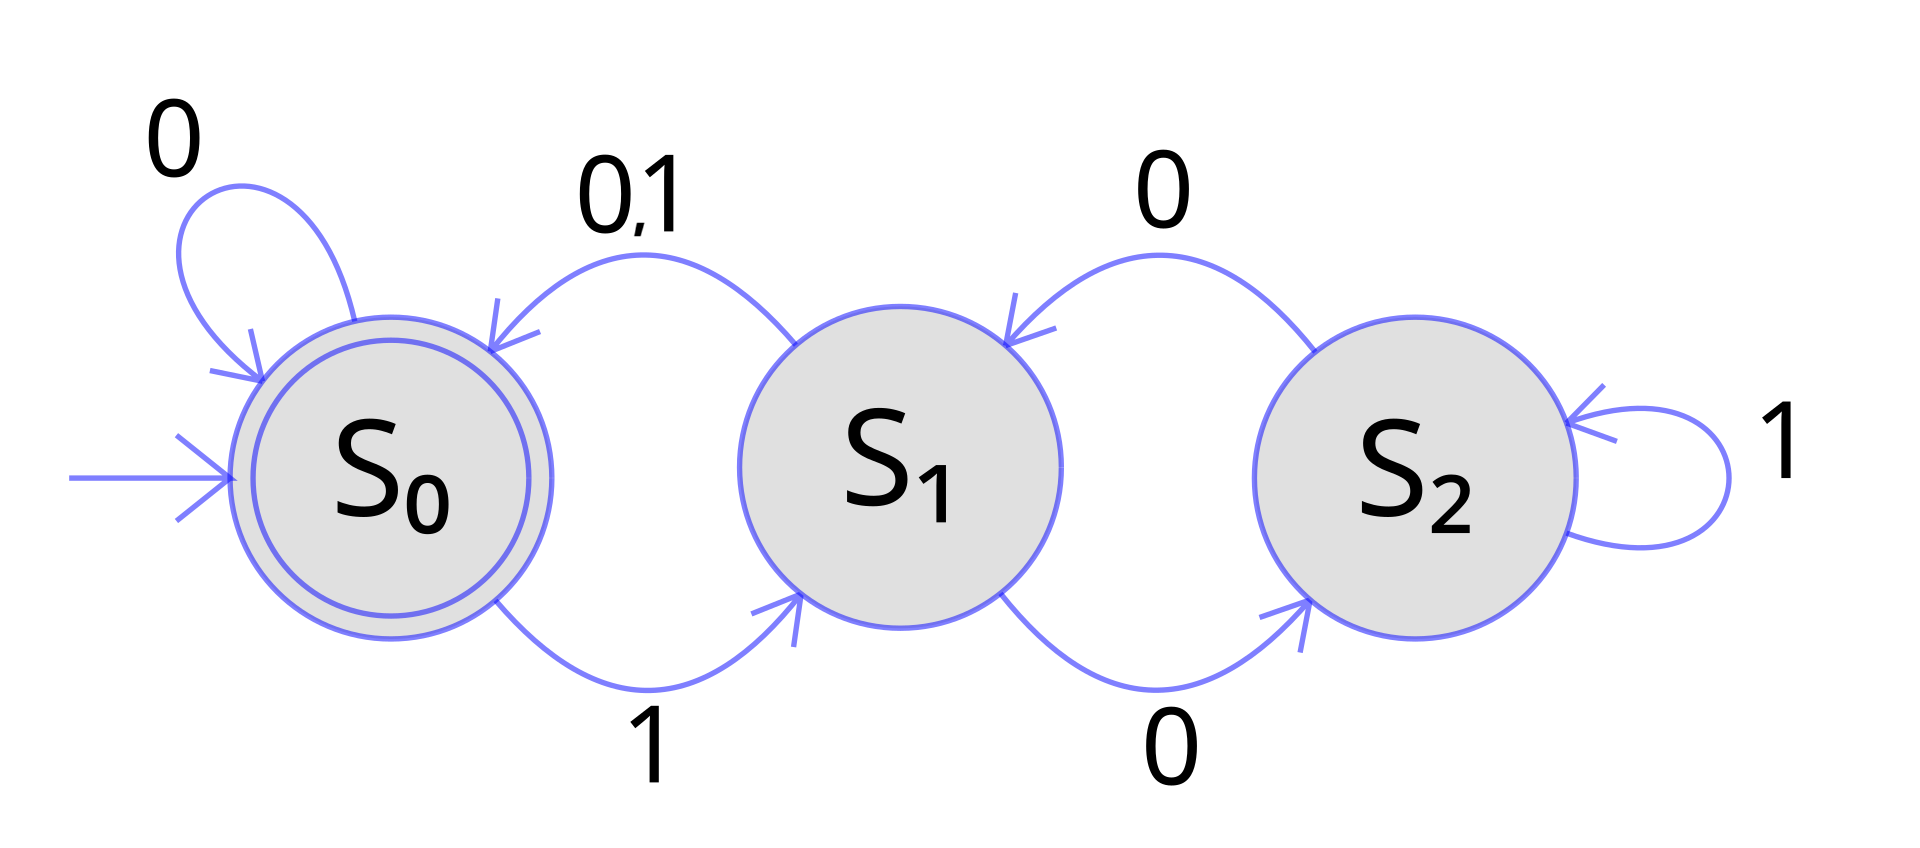
\includegraphics[width=0.6\textwidth]{4. applications/finateStateAutomationsGenNets/images/NDFA.png}
\caption{Пример за недетерминиран краен автомат.}
\label{fig:nfa_figure}
\end{figure}

\paragraph{Кога НКА приема дума?}
\mbox{}\\
Нека $\alpha = a_0 a_1 \cdots a_{n-1} \in \Sigma^*$ е дума. Недетерминираният краен автомат
$\mathcal{N}$ \emph{приема} $\alpha$, ако съществува последователност от състояния
$q_0, q_1, \dots, q_n$, такава че:
\begin{itemize}
	\item $q_0 = q_{\textit{start}}$;
	\item за всяко $i$ с $0 \le i < n$ е изпълнено $q_{i+1} \in \Delta(q_i, a_i)$;
	\item $q_n \in F$.
\end{itemize}
Еквивалентно, чрез разширената преходна функция
\[
	\Delta^* : \mathcal{P}(Q) \times \Sigma^* \;\longrightarrow\;\mathcal{P}(Q),
\]
се казва, че $\alpha$ е приета тогава и само тогава, когато
\[
	\Delta^*(\{q_{\textit{start}}\}, \alpha) \;\cap\; F \;\neq\; \varnothing.
\]

\paragraph{Език на НКА.}
\mbox{}\\
\emph{Езикът, разпознат} от НКА $\mathcal{N}$, е
\[
	L(\mathcal{N}) \;=\; \{\,\alpha \in \Sigma^* \,\mid\, \text{$\mathcal{N}$ приема $\alpha$}\}.
\]

\medskip

\paragraph*{Сравнение между детерминирани и недетерминирани автомати.}
\label{subsec:comparison_dfa_nfa}
\mbox{}\\
Макар ДКА и НКА да се дефинират по различен начин, те разпознават един и същи клас от езици. По-долу се посочват някои основни разлики и добре известният резултат, който ги свързва:
\begin{itemize}
    \item \textbf{Единствена изчислителна пътека (ДКА).}\\
    При \emph{детерминиран} краен автомат за всяко състояние и входен символ съществува точно едно възможно следващо състояние. При обработка на входен низ ДКА следва \emph{единствена} изчислителна пътека от началното към (възможно) приемащо състояние.

    \item \textbf{Паралелна изчислителност (НКА).}\\
    Обратно, \emph{недетерминираният} краен автомат може да има множество възможни следващи състояния за дадена двойка състояние–символ. НКА може да се разглежда като изследващ \emph{всички възможни} изчислителни пътеки паралелно; ако \emph{някоя} от тях достига приемащо състояние, входът се счита приет. Това разклонено поведение често улеснява конструирането на автомати.

    \item \textbf{Интерпретация на ДКА като НКА.}\\
    \emph{Всеки} ДКА може тривиално да се интерпретира като НКА: функцията на прехода връща \emph{множество с точно един елемент}. Следователно ДКА представляват специален случай на НКА с единствен възможен преход на всяка стъпка.

    \item \textbf{Теорема на Рабин–Скот.} \\
    Важна теорема във формалните езици, доказана от Рабин и Скот \cite{rabin-scott}, гласи, че за всеки НКА съществува еквивалентен ДКА, който разпознава същия език. Тази \emph{еквивалентност} обикновено се демонстрира чрез \emph{конструкцията със степенното множество} (\textit{powerset construction}). Идеята е състоянията на новия ДКА да съответстват на \emph{подмножества} от състоянията на оригиналния НКА, като по този начин се улавят всички възможни недетерминирани преходи по детерминиран начин.

    \item \textbf{Защо НКА често се използват като начална стъпка?} \\
    В много теоретични приложения често е \emph{по-лесно} да се проектира НКА благодарение на гъвкавостта му да допуска множество преходи. След като НКА е зададен, при нужда може систематично да се преобразува в ДКА.
\end{itemize}

\subsubsection{Представяне на недетерминирани крайни автомати чрез обобщени мрежи}
\label{sec:simulating_automata_gn}

\hspace*{2.5em}Както беше споменато по-рано, \emph{ОМ} предоставят гъвкава рамка за симулиране на паралелни процеси \cite{Z1,BAM}, което ги прави подходящи за моделиране на начина, по който думите се приемат от автоматите.  
Тук се показва как един \emph{недетерминиран краен автомат} (НКА) може да бъде представен като ОМ.  
Тъй като всеки \emph{детерминиран краен автомат} (ДКА) може лесно да се разглежда като НКА, същата конструкция се прилага и за ДКА с минимални изменения.  
На \textbf{Фигура~\ref{fig:nfa-aa}} е показан индуциран подавтомат, който по-късно се използва като пример.

\begin{figure}[htbp]
	\centering
	\begin{tikzpicture}[>=stealth, scale=1.75]
		% Възли
		\node[circle, draw, minimum size=0.5cm] (A) at (0,0) {$q_1$};
		\node[circle, draw, minimum size=0.5cm] (B) at (2,-1) {$q_2$};
		\node[circle, draw, minimum size=0.5cm] (C) at (2,1) {$q_3$};
		
		% Стрелка към състояние 1 (скрит начален възел)
		\draw[->] (-1,0) -- (A);
		
		% Съществуващи стрелки
		\draw[->] (A) -- node[above] {a} (B);
		\draw[->] (A) -- node[above] {a} (C);
	\end{tikzpicture}
	\captionsetup{width=0.7\textwidth}
	\caption{Индуциран подавтомат с две ребра с етикет \emph{a}, изходящи от едно и също състояние.}
	\label{fig:nfa-aa}
\end{figure}

ОМ се конструира така, че да обхваща всички възможни паралелни изчислителни пътеки на дадения НКА.  
Всеки \emph{преход} в мрежата съответства на едно \emph{състояние} на автомата, а всяка \emph{позиция} в мрежата представлява \emph{ребро} (преходно ребро) на автомата.  
Добавят се и допълнителни преходи и позиции, както е описано по-долу.


\paragraph*{Преходи.}

\begin{itemize}
    \item \textbf{Един преход за всяко състояние на автомата.}\\ За всяко състояние \( q_i \) на НКА се дефинира съответният преход \( Z_i \) в ОМ. Концептуално този преход обработва всички движения от състояние \( q_i \) към неговите следващи състояния, определени от преходната функция на автомата.

    \item \textbf{Краен преход.}\\ Освен преходите, които съпоставят всяко състояние с неговите наследници, се въвежда специален \emph{краен преход} \( Z_{\mathit{final}} \). Този преход позволява на едно \emph{ядро} да \emph{напусне} мрежата, след като автоматът е приел входната дума. Крайният преход има множество входни позиции (свързани с преходите, съответстващи на крайните състояния) и една изходна позиция (която не е входна за никой преход). Ако ядро достигне тази позиция, то това сигнализира за приемане на думата.
\end{itemize}

\paragraph*{Позиции.}

\begin{itemize}
    \item \textbf{Ребра като позиции.}\\ Всяко \emph{ребро} на оригиналния НКА се превръща в \emph{позиция} в мрежата.

    \item \textbf{Входни и изходни позиции.}\\ Ребро от състояние \( q_i \) към \( q_j \) се представя като \emph{изходна} позиция на прехода \( Z_{i} \) и \emph{входна} позиция на прехода \( Z_{j} \).

    \item \textbf{Позиции към крайния преход.}\\ За всяко крайно състояние на НКА се добавя допълнителна изходна позиция от съответния преход, което служи за вход към крайния преход \( Z_{\mathit{final}} \).

    \item \textbf{Начална позиция.}\\ Мрежата съдържа специална начална позиция ($p_{start}$), където първоначално се появява ядро. Тази позиция е входна за прехода, съответстващ на началното състояние на НКА.

    \item \textbf{Крайна позиция.}\\ Мрежата съдържа специална финална позиция, която е единствената изходна позиция на крайния преход \( Z_{\mathit{final}} \). Ядра, достигнали тази позиция, обозначават успешно приемане.
\end{itemize}

\paragraph*{Ядра и техните характеристики.}
\mbox{}\\
В ОМ активните обекти, които се движат между позициите, се наричат \emph{ядра}. В тази конструкция всяко ядро съответства на възможна изчислителна пътека в НКА.

\begin{itemize}
    \item \textbf{Остатък от думата като характеристика.}\\ Всяко ядро носи като своя \emph{характеристика} непрочетената част от входната дума, означена като „\texttt{word}“. Първоначално тази характеристика е цялата входна дума \( w = a_0 a_1 \cdots a_{n-1} \).

    \item \textbf{Характеристични функции на позициите.}\\ Всяка изходна позиция на преход в мрежата има характеристична функция, която актуализира непрочетената дума: при преминаване през позиция, различна от началната, първият символ на думата се премахва. За позицията, през която ядро влиза от $p_{start}$, символ не се премахва.

    \item \textbf{Паралелни пътеки.}\\  Ако НКА се разклонява към няколко наследника, ядрото се дублира в няколко копия с еднакъв текущ остатък на думата.

    \item \textbf{Празен низ.}\\ Когато характеристиката „\texttt{word}“ стане празна, целият вход е обработен. Ако ядрото е на изходна позиция, свързана с крайно състояние, то може да премине към крайния преход \( Z_{\mathit{final}} \) и да напусне мрежата, отбелязвайки приемане.
\end{itemize}

\paragraph*{Илюстрация на движението на ядрата.}
\mbox{}\\
Разглежда се примерът от \textbf{Фигура~\ref{fig:nfa-aa}}, където едно състояние на НКА има две ребра с етикет „a“, водещи към различни състояния (например \(q_2\) и \(q_3\)).  
В ОМ ядрото се \emph{разделя} на две ядра, всяко от които носи един и същ остатък от входната дума.  
Нека първоначалната дума е \(a\alpha\) с \(\alpha \in \Sigma^*\). След разделянето двете ядра запазват същия остатък \(a\alpha\).

На \textbf{Фигура~\ref{fig:gn-nfa}} е показана ОМ, съответстваща на индуцирания НКА, в състояние с две активни ядра преди изпълнението на стъпка.
\newpage
\begin{figure}[ht]
  \centering
  \tiny
  \setlength{\unitlength}{16pt}
  \begin{picture}(15.06,9.07)
    \linethickness{0.4pt}
    % --- Transitions ---
    \put(3.18,9.37){\makebox(0,0)[b]{$Z_1$}}
    \put(3.18,8.00){\makebox(0,0)[bb]{\Large$\bigtriangledown$}}
    \put(3.18,8.00){\line(0,-1){8.00}}
    \put(11.89,9.37){\makebox(0,0)[b]{$Z_2$}}
    \put(11.91,8.00){\makebox(0,0)[bb]{\Large$\bigtriangledown$}}
    \put(11.91,8.00){\line(0,-1){3.00}}
    \put(11.89,4.37){\makebox(0,0)[b]{$Z_3$}}
    \put(11.91,3.00){\makebox(0,0)[bb]{\Large$\bigtriangledown$}}
    \put(11.91,3.00){\line(0,-1){3.00}}
    % --- Places ---
    \put(6.33,7.13){\makebox(0,0)[cc]{$p_{1-2}$}}
    \put(6.33,6.33){\circle{1.0}}
    \put(6.33,6.33){\circle*{0.4}}

    \put(6.32,2.46){\makebox(0,0)[cc]{$p_{1-3}$}}
    \put(6.32,1.67){\circle{1.0}}
    \put(6.32,1.67){\circle*{0.4}}
    \put(15.06,7.13){\makebox(0,0)[cc]{$p_{2-y}$}}
    \put(15.06,6.33){\circle{1.0}}
    \put(15.06,2.46){\makebox(0,0)[cc]{$p_{3-z}$}}
    \put(15.06,1.67){\circle{1.0}}
    \put(0.00,4.79){\makebox(0,0)[cc]{$p_{x-1}$}}
    \put(0.00,4.00){\circle{1.0}}
    % --- Edges ---
    % Z1 -> p2
    \put(3.20,6.33){\vector(1,0){2.63}}
    % Z1 -> p3
    \put(3.20,1.67){\vector(1,0){2.62}}
    % Z2 -> p4
    \put(11.94,6.33){\vector(1,0){2.62}}
    % Z3 -> p5
    \put(11.94,1.67){\vector(1,0){2.62}}
    % p1 -> Z1
    \put(0.50,4.00){\vector(1,0){2.65}}
    % p2 -> Z2
    \put(6.83,6.33){\vector(1,0){5.06}}
    % p3 -> Z3
    \put(6.82,1.67){\vector(1,0){5.07}}
  \end{picture}
  \normalsize
  \captionsetup{width=0.8\textwidth}
  \caption{ОМ, съответстваща на индуцирания НКА от \textbf{Фигура~~\ref{fig:nfa-aa}}, с две активни ядра ПРЕДИ стъпка.}
  \label{fig:gn-nfa}
\end{figure}

За имената на позициите се използва конвенцията \( p_{\text{origin-destination}} \).  
При следващото преместване ядрата се придвижват към $p_{2-y}$ и $p_{3-z}$.  
Характеристичните функции на тези позиции премахват първия символ от думата; следователно, и двете ядра ще носят актуализирания остатък \(\alpha\), както е показано на \textbf{Фигура~\ref{fig:gn-nfa-after-step}}.

\begin{figure}[ht]
  \centering
  \tiny
  \setlength{\unitlength}{16pt}
  \begin{picture}(15.06,9.07)
    \linethickness{0.4pt}
    % --- Transitions ---
    \put(3.18,9.37){\makebox(0,0)[b]{$Z_1$}}
    \put(3.18,8.00){\makebox(0,0)[bb]{\Large$\bigtriangledown$}}
    \put(3.18,8.00){\line(0,-1){8.00}}
    \put(11.89,9.37){\makebox(0,0)[b]{$Z_2$}}
    \put(11.91,8.00){\makebox(0,0)[bb]{\Large$\bigtriangledown$}}
    \put(11.91,8.00){\line(0,-1){3.00}}
    \put(11.89,4.37){\makebox(0,0)[b]{$Z_3$}}
    \put(11.91,3.00){\makebox(0,0)[bb]{\Large$\bigtriangledown$}}
    \put(11.91,3.00){\line(0,-1){3.00}}
    % --- Places ---
    \put(6.33,7.13){\makebox(0,0)[cc]{$p_{1-2}$}}
    \put(6.33,6.33){\circle{1.0}}

    \put(6.32,2.46){\makebox(0,0)[cc]{$p_{1-3}$}}
    \put(6.32,1.67){\circle{1.0}}

    \put(15.06,7.13){\makebox(0,0)[cc]{$p_{2-y}$}}
    \put(15.06,6.33){\circle{1.0}}
    \put(15.06,6.33){\circle*{0.4}}
    \put(15.06,2.46){\makebox(0,0)[cc]{$p_{3-z}$}}
    \put(15.06,1.67){\circle{1.0}}
    \put(15.06,1.67){\circle*{0.4}}
    \put(0.00,4.79){\makebox(0,0)[cc]{$p_{x-1}$}}
    \put(0.00,4.00){\circle{1.0}}
    % --- Edges ---
    % Z1 -> p2
    \put(3.20,6.33){\vector(1,0){2.63}}
    % Z1 -> p3
    \put(3.20,1.67){\vector(1,0){2.62}}
    % Z2 -> p4
    \put(11.94,6.33){\vector(1,0){2.62}}
    % Z3 -> p5
    \put(11.94,1.67){\vector(1,0){2.62}}
    % p1 -> Z1
    \put(0.50,4.00){\vector(1,0){2.65}}
    % p2 -> Z2
    \put(6.83,6.33){\vector(1,0){5.06}}
    % p3 -> Z3
    \put(6.82,1.67){\vector(1,0){5.07}}
  \end{picture}
  \normalsize
  \captionsetup{width=0.8\textwidth}
  \caption{ОМ, съответстваща на индуцирания НКА от \textbf{Фигура~~\ref{fig:nfa-aa}}, с две активни ядра СЛЕД стъпка.}
  \label{fig:gn-nfa-after-step}
\end{figure}

\paragraph*{Индексирани матрици.}
\mbox{}\\
По-долу се описва как се конструират \emph{индексираните матрици} на ОМ, която симулира зададен НКА \((Q, \Sigma, \delta, q_{start}, F)\).

\paragraph*{Дефиниция на основен предикат.}
\mbox{}\\
Въвежда се следният предикат, използван в индексираните матрици:
\[
S(x,y)\;\Longleftrightarrow\;
\begin{aligned}
&\text{характеристиката „\textit{Word}“ на ядрото е от вида } aw, 
a \in \Sigma,\; w \in \Sigma^{*} \\[0.4mm]
&\text{и } q_{y} \in \delta(q_{x}, a).
\end{aligned}
\]

Тук $q_x$ съответства на състоянието на НКА, свързано с входната позиция $p_x$ в прехода на ОМ, а $q_y$ е състоянието, свързано с изходната позиция $p_y$. Следователно, предикатът $S(x,y)$ е истина точно когато ядрото на позиция $p_x$ може при вход $a$ да премине в състояние $q_y$ в НКА, като характеристичната дума се обновява от $aw$ до $w$.


\paragraph{Преход $Z_i$ за нефинално състояние $q_i$.}
\mbox{}\\
За всяко състояние $q_i \in Q$ нека \textit{Input}$(q_i)$ е множеството от състояния на НКА, които имат директен преход (ребро) към $q_i$, а \textit{Output}$(q_i)$ – множеството от състояния, към които съществува преход (ребро) от $q_i$.  
В ОМ тези ще съответстват съответно на входните и изходните позиции на прехода $Z_i$.  
Формално, индексираната матрица на $Z_i$ има редове, съответстващи на позициите в \textit{Input}$(q_i)$, и колони, съответстващи на позициите в \textit{Output}$(q_i)$.

Следователно индексираната матрица за прехода $Z_i$ е:

\[
\begin{array}{c|c}
    & p_{i-y} \quad \text{където } q_y \in \textit{Output}(q_i) \\ \hline
p_{x-i} \quad \text{където } q_x \in \textit{Input}(q_i) & S(x,i)
\end{array}
\]


\paragraph{Преход на началното състояние с допълнителна позиция.}
\mbox{}\\
За прехода, който съответства на началното състояние, се въвежда допълнителна позиция $p_{\text{start}}$, от която започва симулацията.  
Всяко ядро в $p_{\text{start}}$ може безусловно да се премести в някоя от позициите, които съответстват на \textit{Output}$(q_{\text{start}})$.  
Следователно в индексираната матрица за прехода на началното състояние има допълнителен ред за $p_{\text{start}}$, в който всички елементи са зададени като $\text{\textit{True}}$:

\[
\resizebox{0.4\textwidth}{!}{$
\begin{array}{c|cccc}
    & \dots &   &   & \dots \\ \hline
\vdots & \ddots & & & \vdots \\[6pt]
p_{\text{start}} & \text{True} & \text{True} & \cdots & \text{True} \\
\end{array}
$}
\]

\paragraph{Допълнителна изходна позиция за крайните състояния.}
\mbox{}\\
За всеки преход $Z_i$, който съответства на крайно състояние $q_i \in F$, се въвежда допълнителна изходна позиция $p_{i,\text{final}}$, която служи като вход към крайния „приемащ“ преход $Z_{\text{final}}$.  
Преминаването от прехода \(Z_i\) към \(p_{i,\text{final}}\) е винаги разрешено (т.е. предикатът е $\text{\textit{True}}$).  
В резултат за всеки такъв $Z_i$ индексираната матрица има допълнителна колона, съответстваща на $p_{i,\text{final}}$, в която всеки елемент (в тази колона) е зададен като $\text{\textit{True}}$:

\begin{center}
\resizebox{0.3\textwidth}{!}{
$\begin{array}{c|ccc}
      & \dots & \dots & p_{i,\text{final}} \\ \hline
\vdots & \ddots & \ddots & \text{True} \\
\vdots & \ddots & \ddots & \vdots      \\
\vdots & \ddots & \ddots & \text{True} \\
\end{array}$
}
\end{center}

\paragraph{Краен преход ($Z_{\text{final}}$).}
\mbox{}\\
Накрая се дефинира глобалният краен преход $Z_{\text{final}}$.  
Този преход взема ядра от позициите $p_{t,\text{final}}$, където $q_t \in F$, и ги премества в една „приемаща“ изходна позиция $P_{\text{final}}$.  
За да бъде входната дума приета от симулацията на НКА, характеристичната дума на ядрото трябва да бъде празна. 
За тази цел се използва предикатът:

\[
E \;\;\Longleftrightarrow\;\; \text{характеристичната „дума“ на ядрото е празна.}
\]

Следователно индексираната матрица за $Z_{\text{final}}$ е:

\begin{center}
\resizebox{0.35\textwidth}{!}{
  $\begin{array}{c|c}
       & P_{\text{final}} \\ \hline
   p_{t,\text{final}} \ (q_t \in F) & E
   \end{array}$
}
\end{center}

Ако предикатът $E$ е изпълнен, ядрото се премества в $P_{\text{final}}$, което показва, че симулираният НКА е приел първоначалната входна дума.

\paragraph*{Поток в обобщената мрежа.}
\begin{enumerate}
    \item \textbf{Инициализация.}\\ Едно ядро влиза в ОМ с характеристика, зададена като цялата входна дума \(\alpha\). Това ядро се поставя във входната позиция на ОМ, която съответства на \emph{началното състояние} на НКА.
    
    \item \textbf{Преходи между състояния.}\\ При всеки преход на ОМ \( Z_q \), логиката на предикатите проверява дали следващият входен символ на ядрото съответства на допустим преход от \( q \) към друго състояние \( q' \). Ако е така, ядрото се премества в съответната \emph{позиция} (която представя реброто \( q \rightarrow q' \)). Характеристичната дума на ядрото се обновява чрез премахване на консумирания символ.
    
    \item \textbf{Разклоняване.}\\ Ако съществуват множество допустими преходи от \( q \) (отразяващи недетерминираността на НКА), от \( Z_q \) могат да излязат няколко ядра  всяко със същата характеристична дума, но водещо към различни последващи преходи в ОМ.
    
    \item \textbf{Приемане.}\\ Ако ядрото има празна характеристична дума и се намира (или може да се премести) в позиция, съответстваща на крайно състояние на НКА, то се насочва към \emph{крайния преход} \( Z_{\mathit{final}} \). Оттам то \emph{излиза} от ОМ, което означава успешно приемане на входната дума.
\end{enumerate}
\hspace*{2.5em}При следването на тези стъпки ОМ ефективно симулира всички възможни изчислителни пътища на НКА паралелно. Следователно думата се приема точно тогава, когато поне едно ядро достигне и премине през крайния преход. Този модел подчертава гъвкавостта на ОМ при симулация не само на чисто \emph{детерминирани} механизми (ДКА), но и на системи, изискващи \emph{паралелно изследване} на състоянията (НКА).

\bigskip
\noindent

\begin{Theorem}\label{thm:nka-om}
Всеки недетерминиран краен автомат (НКА) може да бъде представен чрез съответна обобщена мрежа (ОМ).
\end{Theorem}

\renewcommand{\proofname}{Доказателство}
\begin{proof}
Нека $A$ е произволен НКА, $q_i$ е произволно негово състояние и $q_j$ е такова състояние, че $q_i \in \Delta(q_j,a)$ за някое $a \in \Sigma$.

В гореописаната конструкция разглеждаме прехода в ОМ, който съответства на $q_i$. Предикатът на прехода е изпълнен точно тогава когато характеристиката \texttt{word} започва със символ $a$. Характеристичните функции на позициите, излизащи от прехода, премахват първия символ на \texttt{word}, т.е. преобразуват $aw$ във $w$. Следователно активирането на този преход реализира същата обработка на входната дума, както преходът $q_j \xrightarrow{a} q_i$ в автомата, и съответства точно на поведението на състоянията в НКА.

По \textbf{Теоремата за пълнота на преходите в ОМ} всяка ОМ се получава като обединение на своите преходи; следователно мрежата, получена чрез посочената процедура, е коректно изградена като обединение на съответните преходи и представлява завършен модел \cite{Z1, BAM}.

Следователно всеки НКА може да бъде представен чрез съответна ОМ, което доказва твърдението.
\end{proof}


\subsubsection{Подробен пример за недетерминиран краен автомат, представен като обобщена мрежа}

\hspace*{2.5em}По-долу е показан подробен пример за ОМ, съответстваща на недетерминиран краен автомат (НКА) с две крайни състояния $q_3$ и $q_5$ (\textbf{Фигура~\ref{fig:nka-two-finals}}).

\begin{figure}[H]
\centering
\begin{tikzpicture}[>=Latex, scale=1.75]

    % State q_1
    \node[draw, circle, minimum size=0.5cm, inner sep=0pt] (n1) at (0,4) {};
    \node[below=0.1cm of n1] {$q_1$};

    % State q_2
    \node[draw, circle, minimum size=0.5cm, inner sep=0pt] (n2) at (2,4) {};
    \node[below=0.1cm of n2] {$q_2$};

    % State q_3 (final)
    \node[draw, circle, double, minimum size=0.5cm, inner sep=0pt] (n3) at (4,4) {};
    \node[below=0.1cm of n3] {$q_3$};

    % State q_4
    \node[draw, circle, minimum size=0.5cm, inner sep=0pt] (n4) at (4,6) {};
    \node[below=0.1cm of n4] {$q_4$};

    % State q_5 (final)
    \node[draw, circle, double, minimum size=0.5cm, inner sep=0pt] (n5) at (6,6) {};
    \node[below=0.1cm of n5] {$q_5$};

    % Arrow from nowhere to q_1
    \draw[->] (-1,4) -- (n1);

    % Transitions
    \draw[->, bend left=15] (n1) to node[above] {a} (n2);
    \draw[->] (n2) -- node[below] {b} (n3);
    \draw[->] (n2) -- node[left] {b} (n4);
    \draw[->, bend left=20] (n4) to node[above] {a} (n5);
    \draw[->] (n4) to[out=120,in=60,loop] node[above] {b} (n4);
    \draw[->, bend right=30] (n3) to node[above] {b} (n2);

\end{tikzpicture}
\caption{Примерен НКА с две крайни състояния: $q_3$ и $q_5$.}
\label{fig:nka-two-finals}
\end{figure}
Езикът на този автомат може да бъде представен чрез регулярния израз:
\[
a \,(bb)^* \Bigl(b + b^+\,a\Bigr).
\]

Автоматът е недетерминиран, защото от състояние $q_2$ излизат две ребра с етикет „b“. На \textbf{Фигура~\ref{fig:om-sim}} е представена ОМ, симулираща този автомат.
\newpage

\begin{figure}[htbp]
\centering
\setlength{\unitlength}{12pt}%
{\tiny
	\begin{picture}(30.29,17.27)
	\linethickness{0.4pt}

% --- Transitions (unchanged) ---
\put(3.85,17.77){\makebox(0,0)[b]{$Z_1$}}
\put(3.87,16.38){\makebox(0,0)[bb]{\Large$\bigtriangledown$}}
\put(3.87,16.38){\line(0,-1){3.32}}

\put(9.91,17.77){\makebox(0,0)[b]{$Z_2$}}
\put(9.92,16.38){\makebox(0,0)[bb]{\Large$\bigtriangledown$}}
\put(9.92,16.38){\line(0,-1){6.65}}

\put(15.98,17.77){\makebox(0,0)[b]{$Z_4$}}
\put(15.99,16.38){\makebox(0,0)[bb]{\Large$\bigtriangledown$}}
\put(15.99,16.38){\line(0,-1){6.65}}

\put(22.05,17.77){\makebox(0,0)[b]{$Z_5$}}
\put(22.06,16.38){\makebox(0,0)[bb]{\Large$\bigtriangledown$}}
\put(22.06,16.38){\line(0,-1){3.32}}

\put(28.11,17.77){\makebox(0,0)[b]{$Z_{\text{final}}$}}
\put(28.12,16.38){\makebox(0,0)[bb]{\Large$\bigtriangledown$}}
\put(28.12,16.38){\line(0,-1){6.65}}

\put(15.98,8.55){\makebox(0,0)[b]{$Z_3$}}
\put(15.99,7.15){\makebox(0,0)[bb]{\Large$\bigtriangledown$}}
\put(15.99,7.15){\line(0,-1){6.65}}

% --- Places (unchanged) ---
\put(6.05,15.25){\makebox(0,0)[cc]{$p_{1-2}$}} \put(6.05,14.53){\circle{1}}

\put(12.11,12.47){\makebox(0,0)[cc]{$p_{2-3}$}} \put(12.11,11.77){\circle{1}}

\put(12.11,15.25){\makebox(0,0)[cc]{$p_{2-4}$}} \put(12.11,14.53){\circle{1}}

\put(18.18,15.25){\makebox(0,0)[cc]{$p_{4-5}$}} \put(18.18,14.53){\circle{1}}

\put(18.18,12.47){\makebox(0,0)[cc]{$p_{4-4}$}} \put(18.18,11.77){\circle{1}}

\put(24.25,15.25){\makebox(0,0)[cc]{$p_{5-fin}$}} \put(24.25,14.53){\circle{1}}

\put(30.29,15.25){\makebox(0,0)[cc]{$p_{fin}$}} \put(30.29,14.53){\circle{1}}

\put(18.18,6.01){\makebox(0,0)[cc]{$p_{3-fin}$}} \put(18.18,5.31){\circle{1}}

\put(18.18,3.25){\makebox(0,0)[cc]{$p_{3-2}$}} \put(18.18,2.54){\circle{1}}

\put(0.00,15.25){\makebox(0,0)[cc]{$p_{start}$}}
\put(0.00,14.53){\circle{1}}


% --- From transitions to places ---
%% Z1 -> p1-2
\put(3.87,14.53){\vector(1,0){1.68}}
%% Z2 -> p2-3
\put(9.94,11.77){\vector(1,0){1.67}} % shortened from 1.83
%% Z2 -> p3-3
\put(9.94,14.53){\vector(1,0){1.67}} % shortened from 1.83
%% Z4 -> p4-5
\put(16.01,14.53){\vector(1,0){1.67}} % shortened from 1.83
%% Z4 -> p4-4
\put(16.01,11.77){\vector(1,0){1.67}} % shortened from 1.83
%% Z5 -> p5-fin
\put(22.08,14.53){\vector(1,0){1.67}} % shortened from 1.83
%% Z_final -> p-fin
\put(28.14,14.53){\vector(1,0){1.65}} % shortened from 1.83
%% Z3 -> p3-fin
\put(16.01,5.31){\vector(1,0){1.67}}  % shortened from 1.83
%% Z3 -> p3-2
\put(16.01,2.54){\vector(1,0){1.67}}  % shortened from 1.83

% --- From places to transitions ---
%% p_start -> Z1
\put(0.50,14.53){\line(1,0){1.65}}    % start shifted from 0.33
\put(2.15,14.53){\vector(1,0){1.71}}

%% p1-2 -> Z2
\put(6.55,14.53){\line(1,0){1.65}}    % start shifted from 6.38
\put(8.20,14.53){\vector(1,0){1.71}}

%% p3-2 -> Z2
\put(18.18,2.04){\line(0,-1){2.04}}   % shortened from 2.21
\put(18.18,0.00){\line(-1,0){9.95}}
\put(8.23,0.00){\line(0,1){11.77}}
\put(8.23,11.77){\vector(1,0){1.69}}

%% p2-3 -> Z3
\put(12.11,11.27){\line(0,-1){5.96}}  % start shifted from 11.44
\put(12.11,5.31){\line(1,0){3.79}}
\put(15.90,5.31){\vector(1,0){0.13}}

%% p3-3 -> Z4
\put(12.61,14.53){\vector(1,0){3.37}} % start shifted from 12.44

%% p4-4 -> Z4
\put(18.18,11.27){\line(0,-1){2.04}}  % shortened from 2.21
\put(18.18,9.23){\line(-1,0){3.88}}
\put(14.30,9.23){\line(0,1){2.54}}
\put(14.30,11.77){\vector(1,0){1.69}}

%% p4-5 -> Z5
\put(18.68,14.53){\line(1,0){1.63}}   % start shifted from 18.51
\put(20.31,14.53){\vector(1,0){1.74}}

%% p3-fin -> Z_final
\put(18.68,5.31){\line(1,0){3.38}}    % start shifted from 18.51
\put(22.06,5.31){\line(0,1){6.46}}
\put(22.06,11.77){\vector(1,0){6.05}}

%% p5-fin -> Z_final
\put(24.75,14.53){\vector(1,0){3.35}} % start shifted from 24.58

\end{picture}
}

\caption{Обобщена мрежа, която симулира дадения автомат.}
\label{fig:om-sim}
\end{figure}

Както беше описано, има по един преход за всяко състояние ($Z_1, Z_2, Z_3, Z_4, Z_5$) и един допълнителен краен преход ($Z_{\text{final}}$).

\subsubsection{Симулация на множество недетерминирани крайни автомати чрез една обобщена мрежа}

\hspace*{2.5em}В този подраздел се показва, че краен набор от недетерминирани крайни автомати (НКА) може да бъде представена чрез една ОМ.  
Тази форма на представяне позволява едновременно проверяване на входни низове през множество НКА чрез една единствена ОМ.

\begin{Observation}
Всяко крайно множество от НКА може да бъде представено чрез една обобщена мрежа.
\end{Observation}

\renewcommand{\proofname}{Доказателство}
\begin{proof}
Беше показано, че всеки отделен НКА може да бъде симулиран чрез съответна ОМ.  
Освен това, според една теорема, ако $E_1$ и $E_2$ са ОМ, то тяхното обединение $E_1 \cup E_2$ също е ОМ~\cite{Z1}.  
Следователно, чрез обединяване на ОМ, съответстващи на всеки НКА от крайното множество, се получава една ОМ, която представя съвкупно всички разглеждани НКА.
\end{proof}

\subsubsection{Симулация на един недетерминиран краен автомат с помощта на \textit{OnlineGN}}
\label{subsec:simulation_steps}

\hspace*{2.5em}В този пример беше представен НКА и беше построена съответната ОМ, която разпознава език, съдържащ думата \texttt{abbba}.  
По-долу се демонстрира как да стартираме тази ОМ в инструмента \textit{OnlineGN}.  
В симулацията се използва леко изменена нотация (тъй като долни индекси не се поддържат).  
Например, $q_{i-j}$ се изписва като \texttt{qi-j}.

\begin{figure}[H]
	\centering
	\setlength{\fboxrule}{2pt}
	\setlength{\fboxsep}{0pt}
	\fbox{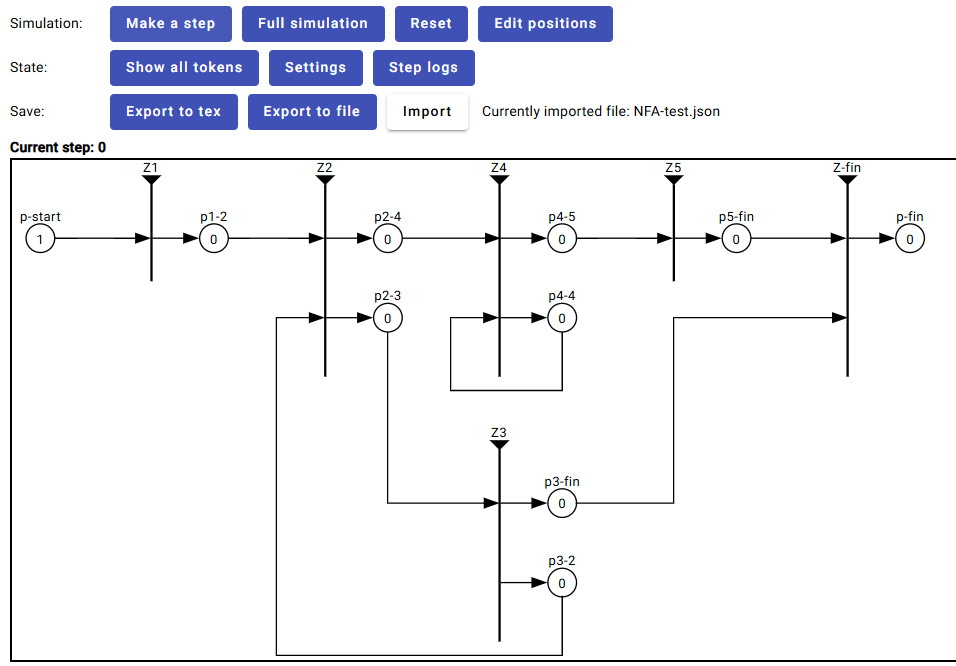
\includegraphics[width=1\textwidth]{4. applications/finateStateAutomationsGenNets/images/NFA-OGN-1.PNG}}
	\caption{Начална конфигурация на ОМ с едно ядро в началната позиция (\texttt{p-start}).}
	\label{fig:gn_initial_setup}
\end{figure}

\vspace{0.2cm}

Както е показано на \textbf{Фигура~\ref{fig:gn_initial_setup}}, ОМ започва с едно ядро в началната позиция \texttt{p-start}.
Началното ядро, носещо пълната входна дума \texttt{abbba}, е показано на \textbf{Фигура~\ref{fig:gn_token_start}}.


\begin{figure}[H]
	\centering
	\setlength{\fboxrule}{2pt}
	\setlength{\fboxsep}{0pt}
	\fbox{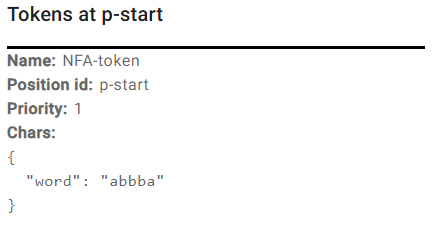
\includegraphics[width=0.6\textwidth]{4. applications/finateStateAutomationsGenNets/images/NFA-OGN-2.PNG}}
	\caption{Ядро в \texttt{p-start} с характеристика \texttt{abbba}.}
	\label{fig:gn_token_start}
\end{figure}

При първата стъпка от симулацията ядрото преминава от \texttt{p-start} към позиция \texttt{p1-2} (вж. \textbf{Фигури~\ref{fig:gn_first_transition}} и~\textbf{\ref{fig:gn_first_transition_zoom}}).  
Отбелязва се, че характеристиката на ядрото остава непроменена след това начално преместване, тъй като обработката на входните символи (т.е. премахването на символи) все още не е започнала.


\begin{figure}[H]
	\centering
	\setlength{\fboxrule}{2pt}
	\setlength{\fboxsep}{0pt}
	\fbox{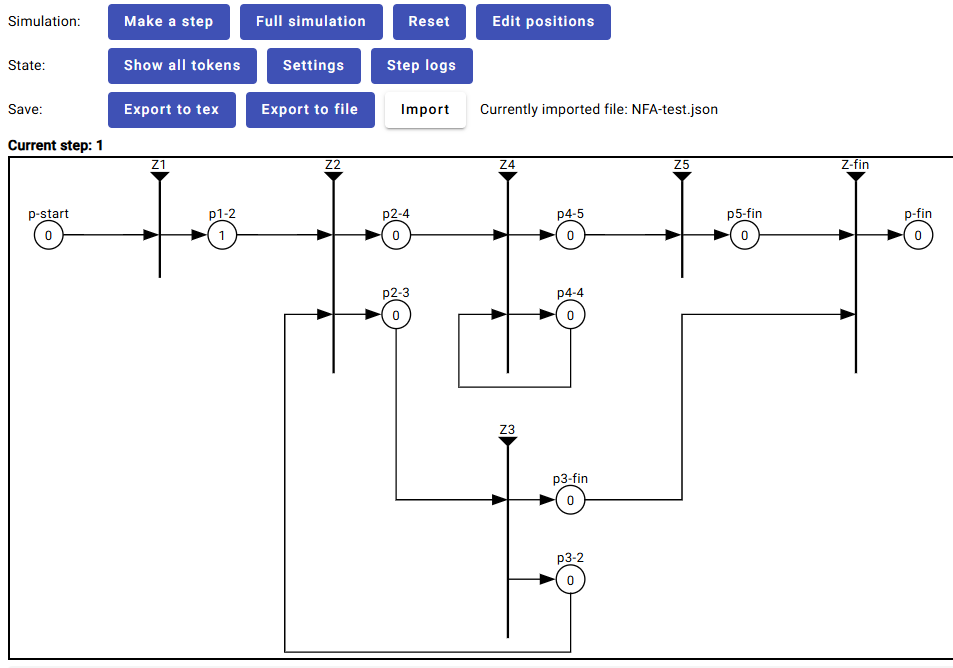
\includegraphics[width=1\textwidth]{4. applications/finateStateAutomationsGenNets/images/NFA-OGN-3.PNG}}
	\caption{След първата стъпка ядрото е в \texttt{p1-2}.}
	\label{fig:gn_first_transition}
\end{figure}


\begin{figure}[H]
	\centering
	\setlength{\fboxrule}{2pt}
	\setlength{\fboxsep}{0pt}
	\fbox{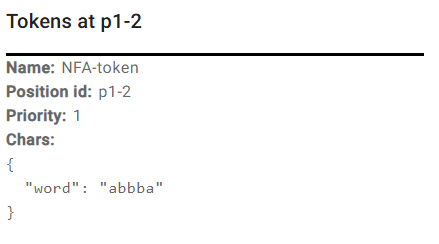
\includegraphics[width=0.6\textwidth]{4. applications/finateStateAutomationsGenNets/images/NFA-OGN-4.PNG}}
	\captionsetup{width=0.8\textwidth}
	\caption{Увеличен изглед на ядрото в \texttt{p1-2}, все още с характеристика \texttt{abbba}.}
	\label{fig:gn_first_transition_zoom}
\end{figure}

Следващите стъпки в ОМ съответстват на последователно прочитане на всеки символ от думата \texttt{abbba} и преминаване през съответните преходи.  
Накрая, след като всички символи бъдат прочетени, ядрото се насочва към крайната позиция \texttt{p-fin}, както е показано на \textbf{Фигура~\ref{fig:gn_final_state}}.

\begin{figure}[H]
	\centering
	\setlength{\fboxrule}{2pt}
	\setlength{\fboxsep}{0pt}
	\fbox{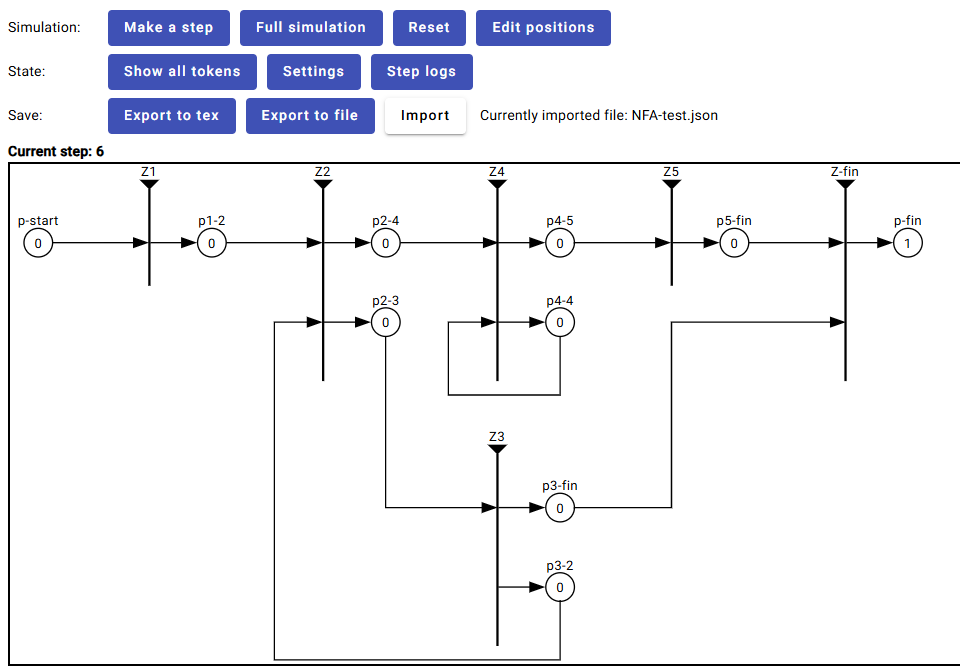
\includegraphics[width=1\textwidth]{4. applications/finateStateAutomationsGenNets/images/NFA-OGN-5.PNG}}
	\caption{Ядрото е достигнало крайната позиция \texttt{p-fin}.}
	\label{fig:gn_final_state}
\end{figure}

Когато ядрото достигне крайната позиция \texttt{p-fin}, неговата характеристика става празен низ, което показва, че цялата дума \texttt{abbba} е разпозната (или „приета“) от ОМ/\linebreak НКА, както е показано на \textbf{Фигура~\ref{fig:gn_empty_characteristic}}.

\begin{figure}[H]
	\centering
	\setlength{\fboxrule}{2pt}
	\setlength{\fboxsep}{0pt}
	\fbox{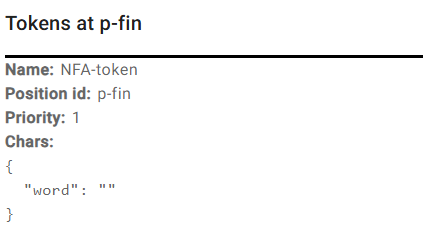
\includegraphics[width=0.6\textwidth]{4. applications/finateStateAutomationsGenNets/images/NFA-OGN-6.PNG}}
	\captionsetup{width=0.7\textwidth}
	\caption{Характеристиката на ядрото става празен низ при приемане.}
	\label{fig:gn_empty_characteristic}
\end{figure}

Тази поредица от стъпки демонстрира как инструментът \textbf{\textit{OnlineGN}} може да се използва за визуализиране и проследяване на движението на ядрата и развитието на техните характеристики (входните символи) през ОМ, моделираща НКА.

\subsubsection{Заключение}

\hspace*{2.5em}В тази глава беше представено как ОМ могат да бъдат използвани за симулация както на детерминирани, така и на недетерминирани крайни автомати.  
Чрез свързване на всяко състояние от автомата с преход в ОМ и представяне на ребрата като позиции, ефективно се улавят всички паралелни изчислителни пътища, които един НКА може да следва.

Архитектурата, базирана на ядра, позволява лесно моделиране на разклонения и едновременна обработка на множество състояния.  
Този подход демонстрира гъвкавостта и устойчивостта на ОМ в теорията на формалните езици и изчисленията, базирани на автомати, като открива възможности за бъдещи приложения в области, където паралелната обработка и конкурентността имат съществена роля.

\input{4. applications/hanoiTowers/hanoiTowers}

\subsection{Модел с обобщена мрежа на производството на газови и полимерни продукти в нефтопреработвателна рафинерия}

\paragraph{Декларация за принос (съвместна публикация).}
\mbox{}\\
Настоящият раздел представя резултати, публикувани в съвместна статия \cite{Stratiev2023_1}.
Приносът на докторанта включва: (i) активно участие в съставянето на ОМ по описанието на процеса;
(ii) реализиране и провеждане на цялостната симулация чрез \textbf{\textit{OnlineGN}}, с което се верифицира моделът,
както и обработка/представяне на резултатите; (iii) подготовка и включване на всички фигури от симулациите и
описание на симулационния процес в текста на раздела.

В тази глава се представя ОМ модел на производството на газови и полимерни нефтопреработвателни продукти и неговата програмна симулация чрез \textit{OnlineGN}. Изграждането на модела и детайлите по формализацията са разгледани подробно в гореспомената статия ~\cite{Stratiev2023_1}.

\subsubsection{Увод в производството на продукти в нефтопреработвателна рафинерия}

\hspace*{2.5em}Моделирането на процесите на производство на рафинирани продукти в нефтопреработвателна рафинерия е полезен инструмент за производствено планиране, тъй като подпомага повишаването на ефективността и рентабилността на производството.

В литературата се срещат частични модели на разнообразните процеси в химическата индустрия и нефтопреработването. Например, в~\cite{Zhou2017} се разглежда оценка на риска в химическата индустрия; в~\cite{Infosys2018} се изследва интегрирането на инженерни модели с планови модели; в~\cite{40} се акцентира върху планирането в мащаб „цяла рафинерия“ при неопределеност в търсенето и цените на продуктите. Общата картина показва, че тези подходи третират отделни аспекти на проблема и по-рядко предлагат единна рамка, която да позволява едновременно описание, анализ и симулация на процесите като взаимосвързана система.

Подходът за моделиране на процесите в нефтопреработването чрез ОМ е оригинален, като публикациите в тази насока до момента са дело на част от авторите на~\cite{Stratiev2023_1}. Благодарение на високата изразителна мощ на ОМ, процесите могат да бъдат описани в детайл и да се отразят причинно--следствените зависимости чрез предикатите на преходите и характеристиките на ядрата. Това дава възможност да се обхванат едновременно структурата на процеса, логиката на протичането му и необходимата числова информация за анализ и симулация.

В предишни изследвания~\cite{87,88} е показано, че процесите на производство на автомобилен бензин~\cite{87} и дизелово гориво~\cite{88} в нефтопреработвателна рафинерия могат да бъдат моделирани чрез ОМ. Прегледът на литературата и досегашните резултати показват, че за цялостно представяне на производството на рафинирани продукти е необходимо постепенно да се моделират отделните технологични вериги и впоследствие да се обединят в обща йерархична структура. Апаратът на ОМ улеснява именно такова интегриране, тъй като отделни ОМ модели могат да бъдат трансформирани в подмрежи на по-общ модел.

Настоящата глава се фокусира върху моделирането и симулирането на производството на газово гориво, втечнен петролен газ (ВПГ, на англ. \textit{LPG}), пропилен и полипропилен, които са част от производствената верига за петролни газове, като допълнение към вече разгледаните процеси за автомобилен бензин и дизелово гориво. Целта е да се моделира разглежданата технологична верига в рамките на нефтопреработвателна рафинерия чрез ОМ, след което моделът да се симулира с \textit{OnlineGN} и да се потвърди неговата коректност.


\subsubsection{Технологична схема за производство на газово гориво, втечнен петролен газ, пропилен и полипропилен в нефтопреработвателна рафинерия}

\hspace*{2.5em}Технологичната производствена верига, използвана в рафинерията „ЛУКОЙЛ Нефтохим Бургас“ (ЛНБ) за производство на компонентите и крайните продукти -- газово гориво, втечнен петролен газ (ВПГ), пропилен и полипропилен, които са предмет на настоящото изследване, е представена на \textbf{Фигура~\ref{H}}.

\begin{figure}[H]
	\centering
	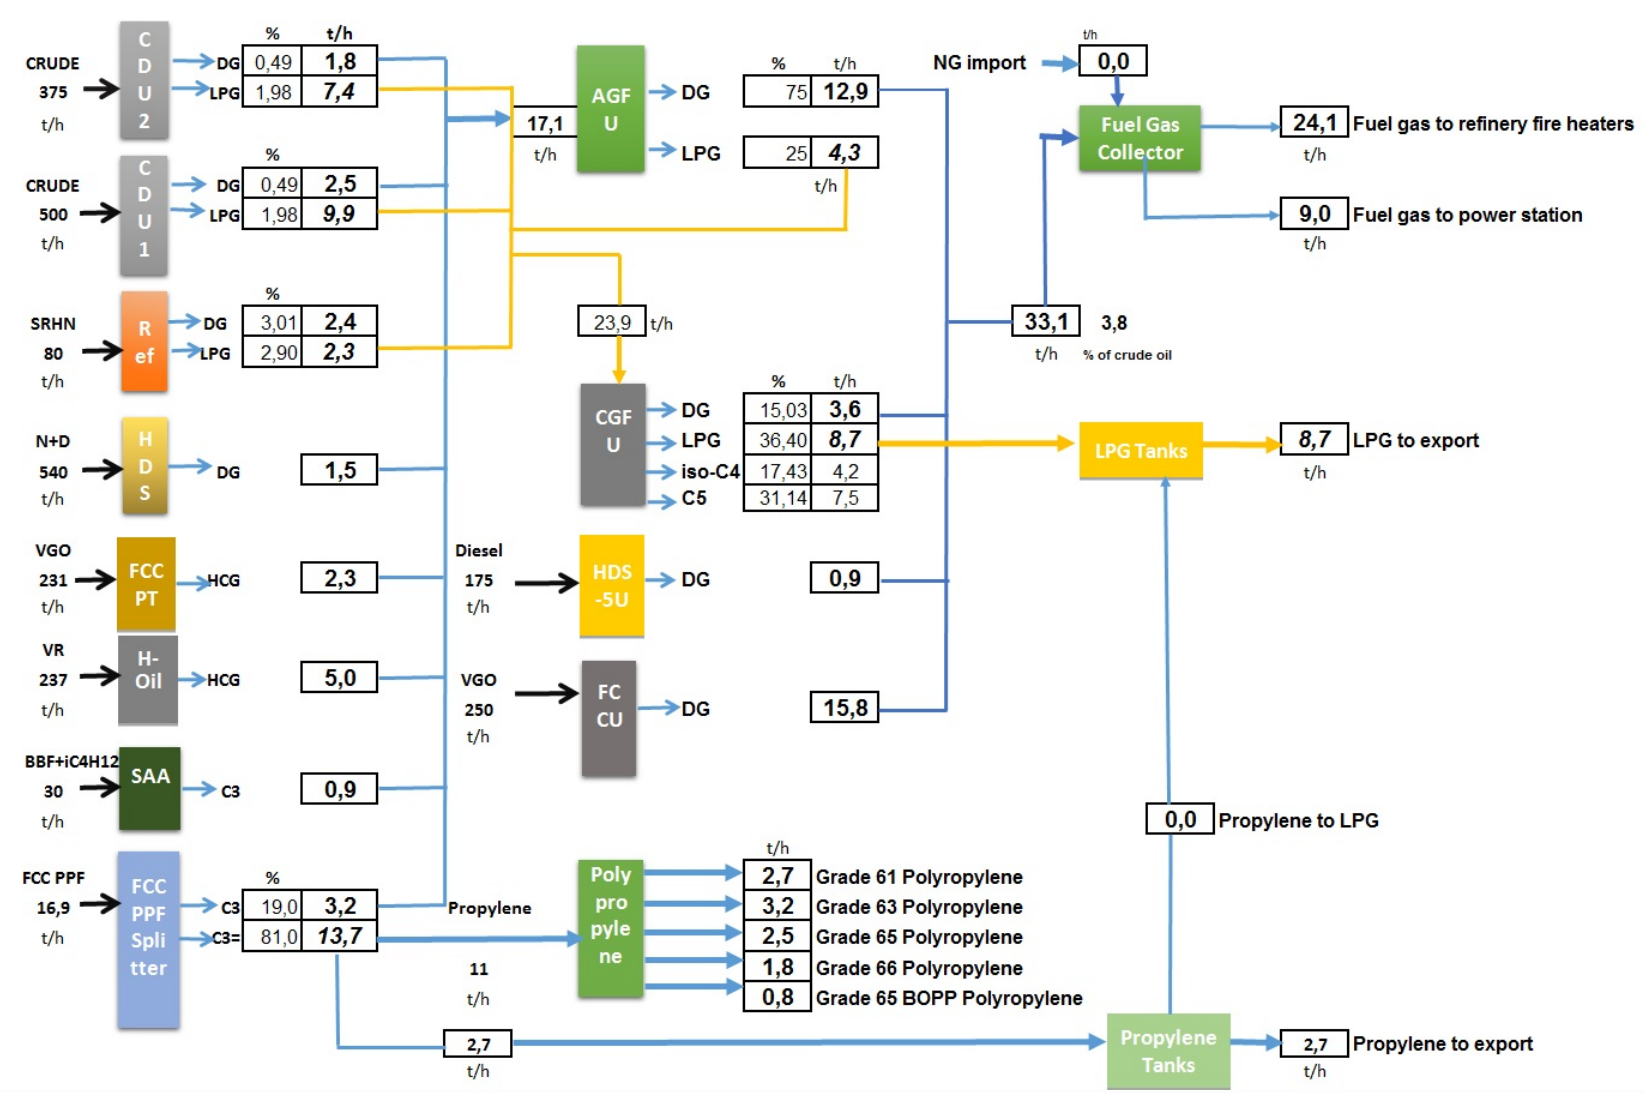
\includegraphics[scale=0.5]{4. applications/fuelGasEtc/images/Figure1.png}
	\caption{Технологична схема за производство на газово гориво, ВПГ, пропилен и полипропилен в нефтопреработвателна рафинерия.}
	\label{H}
\end{figure}

\noindent\textit{Легенда към \textbf{Фигура~\ref{H}} (пояснения на използваните съкращения):}
\begin{itemize}\setlength{\itemsep}{0pt}\setlength{\parskip}{0pt}
	\item \textit{CDU} -- инсталация за атмосферна дестилация на нефта и вакуумна дестилация на атмосферния остатък;
	\item \textit{Ref} -- инсталация за каталитичен реформинг;
	\item \textit{HDS} -- инсталация за хидроочистване на нефтени фракции;
	\item \textit{AGFU} -- инсталация за абсорбация и газофракциониране;
	\item \textit{CGFU} -- централна газофракционираща инсталация;
	\item \textit{HDS-5} -- хидроочистваща инсталация номер 5 от технологичната верига на изследваната рафинерия;
	\item \textit{SAA} -- алкилиране със сярна киселина;
	\item \textit{FCC PPF Splitter} -- ректификационна колона за разделяне на пропан-пропиленовата фракция на пропан и пропилен;
	\item \textit{Polypropylene} -- инсталация за производство на полипропилен чрез полимеризация на пропилен.
\end{itemize}

Тринадесет технологични инсталации в рафинерията участват в производствения процес на газово гориво, ВПГ, пропилен и полипропилен. Количествата на тези петролни газови продукти (в газова и течна фаза), извлечени от суровия нефт при процеса на атмосферна дестилация и генерирани в процесните инсталации -- риформер, хидроочистващи инсталации, \textit{FCC} и \textit{H-Oil} -- в резултат на химични реакции, зависят от произхода на суровия нефт и от експлоатационните режими в посочените инсталации. За случая, показан на \textbf{Фигура~\ref{H}}, производството на газово гориво възлиза на 3.8~\% от количеството суров нефт и повече от половината от него произхожда от флуидното каталитично крекиране (51.8~\%). Друг важен принос за производството на газово гориво има \textit{H-Oil} хидрокрекингът на вакуумен остатък в кипящ слой. Следователно производството на газово гориво е силно зависимо от строгостта на експлоатационните условия, прилагани и в двата процеса за преработка на тежки нефтени фракции -- \textit{FCC} и \textit{H-Oil}. 

Основният източник на ВПГ, както се вижда от данните на \textbf{Фигура~\ref{H}}, е дестилацията на суров нефт. Тя осигурява 75~\% от зареждането на Централната газофракционираща инсталация (\textit{CGFU}), където се извършва извличането на пропан и \textit{n}\,-бутан; тяхното смесване формира рафинирания продукт ВПГ. От \textbf{Фигура~\ref{H}} се вижда, че производството на ВПГ е приблизително четири пъти по-малко от това на газовото гориво. Данните на \textbf{Фигура~\ref{H}} показват, че ако количеството газово гориво е недостатъчно за покриване на енергийните нужди на рафинерията, съществува възможност за внос на природен газ за допълване на наличностите от газово гориво. 

В зависимост от пазарните изисквания течният пропилен може да се експортира като химически сорт за полимеризационен пропилен или да се използва като компонент на продукта ВПГ. Обикновено от инсталацията за полипропилен се произвеждат и изнасят шест сорта полипропиленови продукти.


\subsubsection{Основни резултати: обобщеномрежов модел}

\hspace*{2.5em}ОМ на \textbf{Фигура~\ref{fig3}} съдържа 17 прехода, 55 позиции и 47 типа ядра, съответстващи на следните потоци, продукти и процесни звена:
\begin{itemize}
	\item[$\sigma_1$] ― суров нефт, преработван в \textit{CDU-2}, \textit{t/h}
	\item[$\sigma_2$] ― суров нефт, преработван в \textit{CDU-1}, \textit{t/h}
	\item[$\sigma_3$] ― нафта от пряка дестилация, преработвана в инсталацията за каталитичен реформинг, \textit{t/h}
	\item[$\sigma_4$] ― нафтови и дизелови фракции, преработвани в инсталации за хидрообработка (хидроочистване), \textit{t/h}
	\item[$\sigma_5$] ― вакуумен газьол, преработван в инсталация за хидроочистване на суровината за флуиден каталитичен крекинг (\textit{FCC}), \textit{t/h}
	\item[$\sigma_6$] ― вакуумен остатък, преработван в инсталация за хидрокрекинг по технология \textit{H-Oil}, \textit{t/h}
	\item[$\sigma_7$] ― бутан-бутиленова фракция и изобутен за алкилиране със сярна киселина, \textit{t/h}
	\item[$\sigma_8$] ― пропан-пропиленова фракция от \textit{FCC} за разделяне на пропан и пропилен, \textit{t/h}
	\item[$\sigma_9$] ― първичен и вторичен дизел за хидроочистване в инсталацията \textit{HDS-5}, \textit{t/h}
	\item[$\sigma_{10}$] ― хидроочистен вакуумен газьол и вакуумен газьол от \textit{H-Oil} за преработка във флуиден каталитичен крекинг (\textit{FCC}), \textit{t/h}
	\item[$\sigma_{11}$] ― вносен природен газ за допълване на горивния газ при високо потребление, \textit{t/h}
	
	\item[$\rho_1$] ― инсталация за атмосферна (първична) дестилация на суров нефт \textit{(CDU-2)}
	\item[$\rho_2$] ― инсталация за атмосферна (първична) дестилация на суров нефт \textit{(CDU-1)}
	\item[$\rho_3$] ― инсталация за каталитичен реформинг (каталитичен реформер)
	\item[$\rho_4$] ― инсталации за хидроочистване на нафтови и дизелови фракции
	\item[$\rho_5$] ― инсталация за хидроочистване на суровината за \textit{FCC} (\textit{FCC feed hydrotreater})
	\item[$\rho_6$] ― инсталация за хидрокрекинг на вакуумен остатък по технология \textit{H-Oil}
	\item[$\rho_7$] ― инсталация за алкилиране със сярна киселина
	\item[$\rho_8$] ― инсталация за разделяне на пропан-пропиленова фракция от \textit{FCC} (\textit{FCC PPF splitter})
	\item[$\rho_9$] ― инсталация за абсорбация и газофракциониране (\textit{AGFU})
	\item[$\rho_{10}$] ― междинен резервоар за \textit{LPG} (ВПГ) за събиране на суровина за централната газофракционираща инсталация (\textit{CGFU})
	\item[$\rho_{11}$] ― инсталация за хидроочистване на дизелово гориво \textit{(HDS-5)}
	\item[$\rho_{12}$] ― инсталация за флуиден каталитичен крекинг (\textit{FCC})
	\item[$\rho_{13}$] ― централна газофракционираща инсталация (\textit{CGFU})
	\item[$\rho_{14}$] ― резервоарен парк за \textit{LPG} (ВПГ)
	\item[$\rho_{15}$] ― резервоарен парк за горивен газ
	
	\item[$\alpha_1$] ― ВПГ (\textit{LPG}) продукт от \textit{CDU-2}, \textit{t/h}
	\item[$\alpha_2$] ― ВПГ (\textit{LPG}) продукт от \textit{CDU-1}, \textit{t/h}
	\item[$\alpha_3$] ― ВПГ (\textit{LPG}) продукт от инсталацията за каталитичен реформинг, \textit{t/h}
	\item[$\alpha_4$] ― ВПГ (\textit{LPG}) продукт от \textit{AGFU}, \textit{t/h}
	\item[$\alpha_5$] ― суровина за \textit{CGFU}, \textit{t/h}
	\item[$\alpha_6$] ― ВПГ (\textit{LPG}) продукт от \textit{CGFU} към резервоарния парк, \textit{t/h}
	
	\item[$\beta$]  ― горивен газ за захранване на \textit{AGFU}, \textit{t/h}
	\item[$\beta_1$] ― горивен газ продукт от \textit{CDU-2}, \textit{t/h}
	\item[$\beta_2$] ― горивен газ продукт от \textit{CDU-1}, \textit{t/h}
	\item[$\beta_3$] ― горивен газ продукт от инсталацията за каталитичен реформинг, \textit{t/h}
	\item[$\beta_4$] ― горивен газ продукт от инсталациите за хидроочистване на нафтови и дизелови фракции, \textit{t/h}
	\item[$\beta_5$] ― горивен газ продукт от инсталацията за хидроочистване на суровината за \textit{FCC}, \textit{t/h}
	\item[$\beta_6$] ― горивен газ продукт от инсталацията \textit{H-Oil} за хидрокрекинг на вакуумен остатък, \textit{t/h}
	\item[$\beta_7$] ― пропанова фракция от инсталацията за алкилиране със сярна киселина, \textit{t/h}
	\item[$\beta_8$] ― сух горивен газ продукт от \textit{AGFU}, \textit{t/h}
	\item[$\beta_9$] ― сух горивен газ продукт от \textit{CGFU}, \textit{t/h}
	\item[$\beta_{10}$] ― сух горивен газ продукт от \textit{HDS-5}, \textit{t/h}
	\item[$\beta_{11}$] ― сух горивен газ продукт от \textit{FCC}, \textit{t/h}
	
	\item[$\gamma_1$] ― пропан продукт от \textit{FCC PPF splitter}, \textit{t/h}
	\item[$\gamma_2$] ― пропиленов продукт от \textit{FCC PPF splitter} за захранване на инсталация за полипропилен, \textit{t/h}
	\item[$\gamma_3$] ― пропиленов продукт от \textit{FCC PPF splitter}, \textit{t/h}
	
	\item[$\delta_1$] ― полипропилен, марка 61 (висок индекс на топене), \textit{t/h}
	\item[$\delta_2$] ― полипропилен, марка 63 (висок индекс на топене), \textit{t/h}
	\item[$\delta_3$] ― полипропилен, марка 65 (висок индекс на топене), \textit{t/h}
	\item[$\delta_4$] ― полипропилен, марка 66 (висок индекс на топене), \textit{t/h}
	\item[$\delta_5$] ― полипропилен, марка 65 \textit{BOPP} (висок индекс на топене), \textit{t/h}
	
	\item[$\epsilon_1$] ― ВПГ (\textit{LPG}) продукт за износ, \textit{t/h}
	\item[$\epsilon_2$] ― горивен газ продукт за захранване на електроцентралата на рафинерията, \textit{t/h}
	\item[$\epsilon_3$] ― горивен газ продукт за захранване на процесните пещи на рафинерията, \textit{t/h}
\end{itemize}

\vspace*{-0.85em}

$$Z_1 = \langle\{l_1, l_{11} \}, \{l_{9}, l_{10}, l_{11} \},
\begin{array}{c|ccc}
	& l_{9} & l_{10} & l_{11} \\ \hline
	l_{1}  & false & false & true \\
	l_{11}  & W_{11,9} & W_{11,10} & true
\end{array} \rangle,$$
където: \\
$W_{11,9} = $ „има заявка за продукт ВПГ от \textit{CDU-2}“;\\
$W_{11,10} = $ „има заявка за продукт горивен газ от \textit{CDU-2}“; 

\vspace{0.10cm}

\noindent
Ядрото $\sigma_1$ влиза в позиция $l_{11}$ и се обединява с ядрото $\rho_1$, получавайки характеристика:
$$„\mbox{текущо количество суров петрол в \textit{CDU-2}}“.$$

\vspace{-0.5em}

В следващата времева стъпка ядрото $\rho_1$ се разделя на три ядра - самото $\rho_1$, което остава в $l_{11}$, и ядрата $\alpha_1$ и $\beta_1$.

Ядрото $\alpha_1$ получава характеристика:
$$„\mbox{текущо количество ВПГ продукт от \textit{CDU-2}}“$$
в позиция $l_{9}$, ядрото $\beta_1$ - характеристика:
$$„\mbox{текущо количество горивен газ от \textit{CDU-2}}“$$
в позиция $l_{10}$, а ядрото $\rho_1$ запазва характеристика:
$$„\mbox{текущо количество суров петрол в \textit{CDU-2}}“.\vspace{-0.95em}$$


$$Z_2 = \langle\{l_2, l_{14} \}, \{l_{12}, l_{13}, l_{14} \},
\begin{array}{c|ccc}
	& l_{12} & l_{13} & l_{14} \\ \hline
	l_{2}  & false & false & true \\
	l_{14}  & W_{14,12} & W_{14,13} & true
\end{array} \rangle,$$
където:\\
$W_{14,12} =~$„има заявка за продукт ВПГ от \textit{CDU-1}“;\\
$W_{14,13} =~$„има заявка за продукт горивен газ от \textit{CDU-1}“.

\vspace{0.10cm}

\noindent
Ядрото $\sigma_2$ влиза в позиция $l_{14}$ и се обединява с ядро $\rho_2$, получавайки характеристика:
$$„\mbox{текущо количество суров петрол в \textit{CDU-1}}“.$$

\vspace{-0.5em}

В следващата времева стъпка ядрото $\rho_2$ се разделя на три ядра - самото $\rho_2$, което остава в $l_{14}$, и ядрата $\alpha_2$ и $\beta_2$.

Ядрото $\alpha_2$ получава характеристика:
$$„\mbox{текущо количество ВПГ продукт от \textit{CDU-1}}“$$
в позиция $l_{12}$, ядрото $\beta_2$ - характеристика:
$$„\mbox{текущо количество горивен газ от \textit{CDU-1}}“$$
в позиция $l_{13}$, а ядрото $\rho_2$ запазва характеристика:
$$„\mbox{текущо количество суров петрол в \textit{CDU-1}}“. \vspace{-0.95em}$$


$$Z_3 = \langle\{l_3, l_{17} \}, \{l_{15}, l_{16}, l_{17} \},
\begin{array}{c|ccc}
	& l_{15} & l_{16} & l_{17} \\ \hline
	l_{3}  & false & false & true \\
	l_{17}  & W_{17,15} & W_{17,16} & true
\end{array} \rangle,$$
където:\\
$W_{17,15} =~$„има заявка за продукт ВПГ от каталитичния реформер“;\\
$W_{17,16} =~$„има заявка за продукт горивен газ от каталитичния реформер“.

\vspace{0.10cm}

\noindent
Ядрото $\sigma_3$ влиза в позиция $l_{17}$ и се обединява с ядро $\rho_3$, получавайки характеристика:
$$„\mbox{текущо количество нафта в каталитичния реформер}“.$$

\vspace{-0.5em}

В следващата времева стъпка ядрото $\rho_3$ се разделя на три ядра - самото $\rho_3$, което остава в $l_{17}$, и ядрата $\alpha_3$ и $\beta_3$.

Ядрото $\alpha_3$ получава характеристика:
$$„\mbox{текущо количество ВПГ продукт от каталитичния реформер}“$$
в позиция $l_{15}$, ядрото $\beta_3$ - характеристика:
$$„\mbox{текущо количество горивен газ от каталитичния реформер}“$$
в позиция $l_{16}$, а ядрото $\rho_3$ запазва характеристика:
$$„\mbox{текущо количество нафта в каталитичния реформер}“. \vspace{-0.95em}$$


$$Z_4 = \langle\{l_4, l_{19} \}, \{l_{18}, l_{19} \},
\begin{array}{c|cc}
	& l_{18} & l_{19} \\ \hline
	l_{4}  & false & true \\
	l_{19}  & W_{19,18} & true
\end{array} \rangle,$$
където:\\
$W_{19,18} =~$„има заявка за продукт горивен газ от нафтовите и дизелови хидроочистватели“.

\begin{figure}[H]
	\centering
	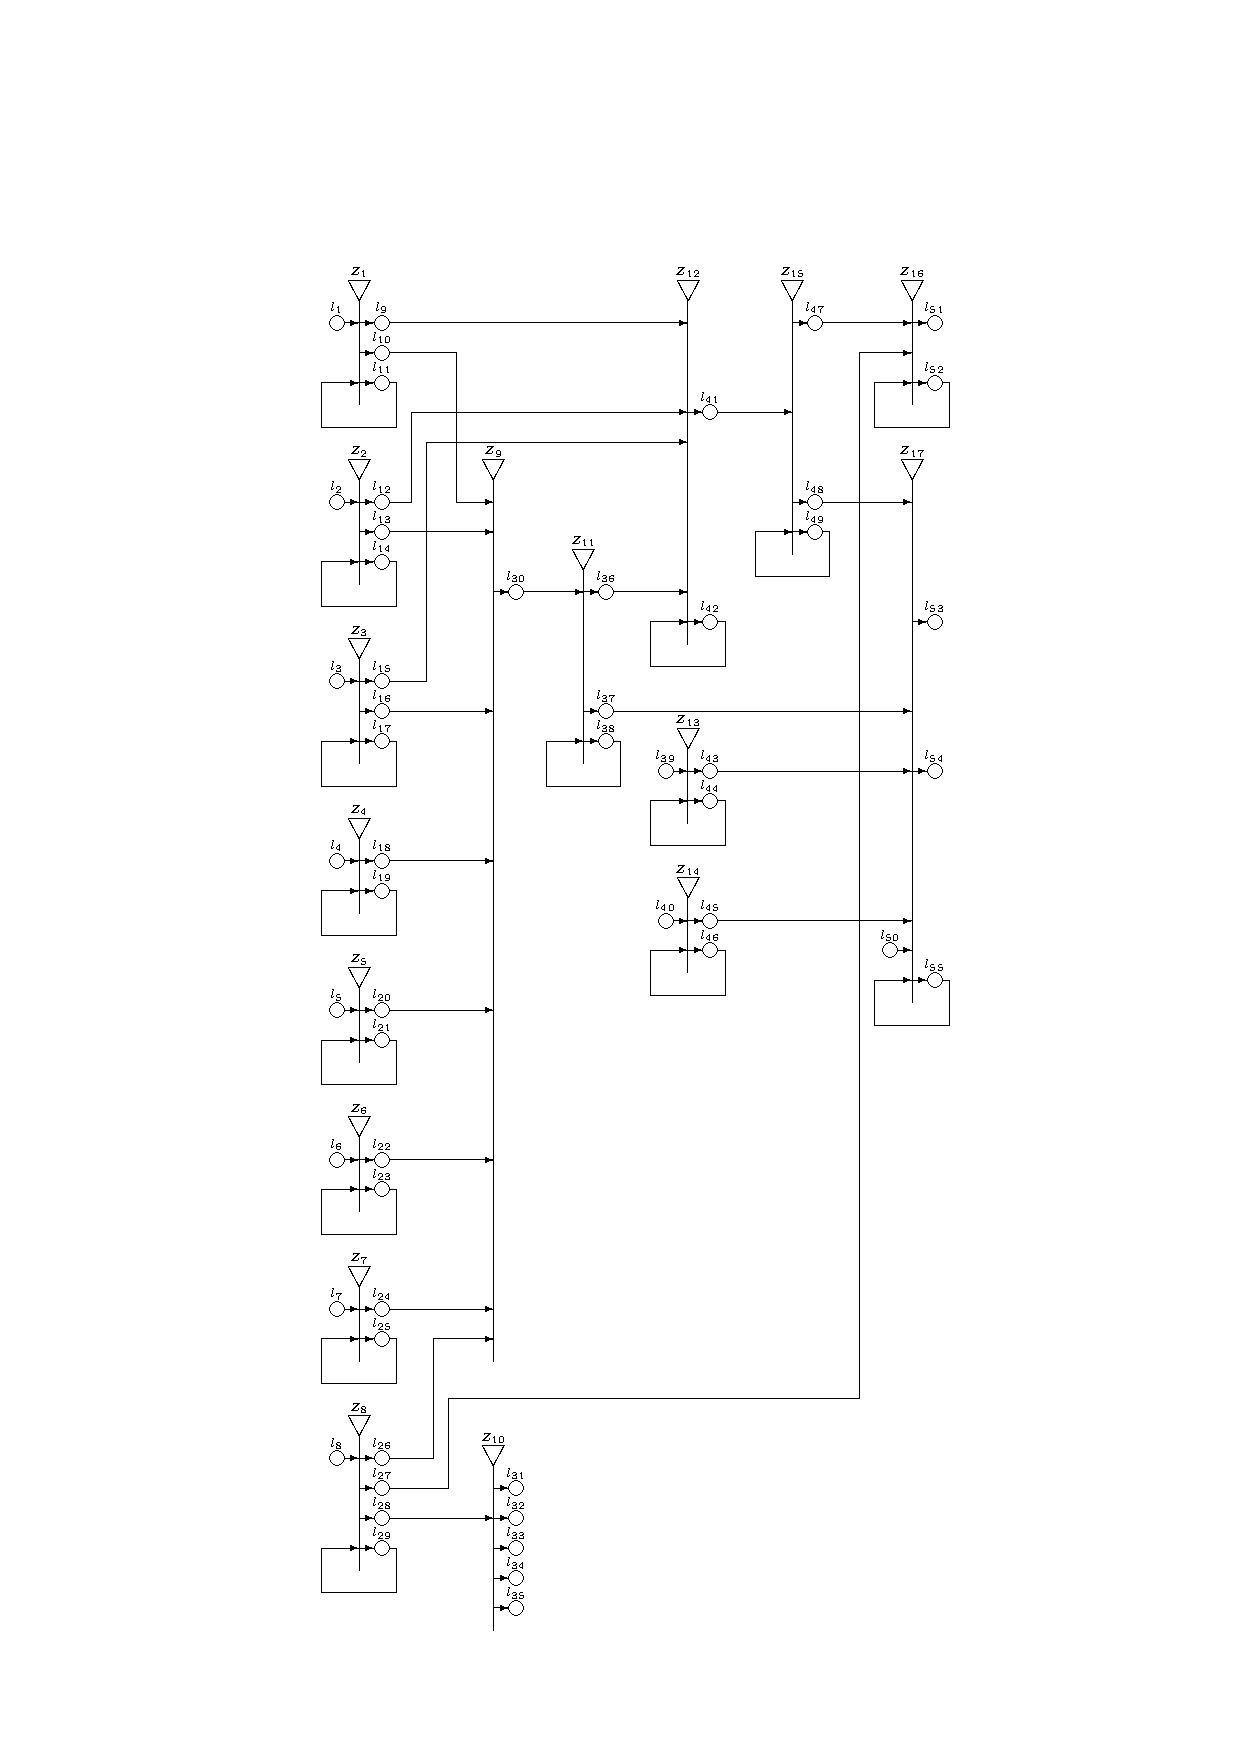
\includegraphics[width=10.3cm]{4. applications/fuelGasEtc/images/Figure3.pdf}
	\caption{ОМ модел.}
	\label{fig3}
\end{figure}


\noindent
Ядрото $\sigma_4$ влиза в позиция $l_{19}$ и се обединява с ядрото $\rho_4$, получавайки характеристика:
$$„\mbox{текущо количество нафта и дизел в нафтовите и дизелови хидроочистватели}“.$$

\vspace{-0.5em}

В следващата времева стъпка ядрото $\rho_4$ се разделя на две ядра - самото $\rho_4$, което остава в $l_{19}$, и ядрото $\beta_4$.

Ядрото $\beta_4$ получава характеристика:
$$„\mbox{текущо количество горивен газ от нафтовите и дизелови хидроочистватели}“$$
в позиция $l_{18}$, а ядрото $\rho_4$ запазва характеристика:
$$„\mbox{текущо количество нафта и дизел в нафтовите и дизелови хидроочистватели}“.$$

\vspace{-0.3em}

$$Z_5 = \langle\{l_5, l_{21} \}, \{l_{20}, l_{21} \},
\begin{array}{c|cc}
	& l_{20} & l_{21} \\ \hline
	l_{5}  & false & true \\
	l_{21}  & W_{21,20} & true
\end{array} \rangle,$$
където:\\
$W_{21,20} =~$„има заявка за продукт горивен газ от хидроочиствателя на хранилка за \textit{FCC}“.

\vspace{0.10em}

\noindent
Ядрото $\sigma_5$ влиза в позиция $l_{21}$ и се обединява с ядрото $\rho_5$, получавайки характеристика:
$$„\mbox{текущо количество вакуумен газьол в хидроочиствателя на хранилка за \textit{FCC}}“.$$

\vspace{-0.5em}

В следващата времева стъпка ядрото $\rho_5$ се разделя на две ядра - самото $\rho_5$, което остава в $l_{21}$, и ядрото $\beta_5$.

Ядрото $\beta_5$ получава характеристика:
$$„\mbox{текущо количество горивен газ в хидроочиствателя на хранилка за \textit{FCC}}“$$
в позиция $l_{20}$, а ядрото $\rho_5$ запазва характеристика:
$$„\mbox{текущо количество вакуумен газьол в хидроочиствателя на хранилка за \textit{FCC}}“.$$

\vspace{-0.3em}

$$Z_6 = \langle\{l_6, l_{23} \}, \{l_{22}, l_{23} \},
\begin{array}{c|cc}
	& l_{22} & l_{23} \\ \hline
	l_{6}  & false & true \\
	l_{23}  & W_{23,22} & true
\end{array} \rangle,$$
където:\\
$W_{23,22} =~$„има заявка за продукт горивен газ от \textit{H-Oil}“.

\vspace{0.1em}

\noindent
Ядрото $\sigma_6$ влиза в позиция $l_{23}$ и се обединява с ядрото $\rho_6$, получавайки характеристика:
$$„\mbox{текущо количество вакуумен остатък в \textit{H-Oil}}“.$$

\vspace{-0.5em}

В следващата времева стъпка ядрото $\rho_6$ се разделя на две ядра - самото $\rho_6$, което остава в $l_{23}$, и ядрото $\beta_6$.

Ядрото $\beta_6$ получава характеристика:
$$„\mbox{текущо количество горивен газ от \textit{H-Oil}}“$$
в позиция $l_{22}$, а ядрото $\rho_6$ запазва характеристика:
$$„\mbox{текущо количество вакуумен остатък в \textit{H-Oil}}“.$$
\vspace{-0.3em}
$$Z_7 = \langle\{l_7, l_{25} \}, \{l_{24}, l_{25} \},
\begin{array}{c|cc}
	& l_{24} & l_{25} \\ \hline
	l_{7}  & false & true \\
	l_{25}  & W_{25,24} & true
\end{array} \rangle,$$
където:\\
$W_{25,24} =~$„има заявка за продукт пропанова фракция от алкилирането със сярна киселина“.

\vspace{0.1em}

\noindent
Ядрото $\sigma_7$ влиза в позиция $l_{25}$ и се обединява с ядро $\rho_7$, получавайки характеристика:
$$„\mbox{текущо количество бутан-бутиленова фракция и изобутан в алкилирането със сярна киселина}“.$$
\vspace{-0.5em}
В следващата времева стъпка ядрото $\rho_7$ се разделя на две ядра - самото $\rho_7$, което остава в $l_{25}$, и ядро $\beta_{7}$.

Ядрото $\beta_{7}$ получава характеристика:
$$„\mbox{текущо количество пропанова фракция в алкилирането със сярна киселина}“$$
в позиция $l_{24}$, а ядрото $\rho_7$ запазва характеристика:
$$„\mbox{текущо количество бутан-бутиленова фракция и изобутан в алкилирането със сярна киселина}“.$$
\vspace{-0.3em}
$$Z_8 = \langle\{l_8, l_{29} \}, \{l_{26}, l_{27}, l_{28}, l_{29} \},
\begin{array}{c|cccc}
	& l_{26} & l_{27} & l_{28} & l_{29} \\ \hline
	l_{8}  & false & false & false & true \\
	l_{29}  & W_{29,26} & W_{29,27} & W_{29,28} & true
\end{array} \rangle,$$
където:\\
$W_{29,26} =~$„има заявка за пропанов продукт от \textit{FCC PPF splitter} за производство на ВПГ“;\\
$W_{29,27} =~$„има заявка за пропилен за полимеризация от \textit{FCC PPF splitter}“;\\
$W_{29,28} =~$„има заявка за пропиленов продукт от \textit{FCC PPF splitter} за износ“.

\vspace{0.1em}

\noindent
Ядрото $\sigma_8$ влиза в позиция $l_{29}$ и се обединява с ядро $\rho_8$, получавайки характеристика:
$$„\mbox{текущо количество \textit{FCC PPF} във \textit{FCC PPF splitter}}“.$$

\vspace{-0.5em}

В следващата времева стъпка ядрото $\rho_8$ се разделя на четири ядра - самото $\rho_8$, което остава в $l_{29}$, и ядрата $\gamma_{1}$, $\gamma_{2}$ и $\gamma_{3}$.

Ядрата $\gamma_{1}$, $\gamma_{2}$ и $\gamma_{3}$ получават съответно характеристики:
$$„\mbox{текущо количество пропанов продукт във \textit{FCC PPF splitter}}“$$
в позиция $l_{26}$,
$$„\mbox{текущо количество пропиленов продукт за полимеризация във \textit{FCC PPF splitter}}“$$
в позиция $l_{27}$,
$$„\mbox{текущо количество пропиленов продукт за износ във \textit{FCC PPF splitter}}“$$
в позиция $l_{28}$, а ядрото $\rho_8$ запазва характеристика:
$$„\mbox{текущо количество \textit{FCC PPF} във \textit{FCC PPF splitter}}“.$$

\vspace{-0.3em}

$$Z_9 = \langle\{l_{10}, l_{13}, l_{16}, l_{18}, l_{20}, l_{22}, l_{24}, l_{26}\}, \{l_{30}\},
\begin{array}{c|c}
	& l_{30} \\ \hline
	l_{10} & true \\
	l_{13} & true \\
	l_{16} & true \\
	l_{18} & true \\
	l_{20} & true \\
	l_{22} & true \\
	l_{24} & true \\
	l_{26} & true
\end{array} \rangle.$$

\noindent
Всички $\beta$-ядра се обединяват в позиция $l_{30}$ в едно ядро $\beta$ с характеристика:
$$„\mbox{текущо количество горивен газ - захранване за \textit{AGFU}}“.$$

\vspace{-0.3em}

$$Z_{10} = \langle\{l_{28}\}, \{l_{31}, l_{32}, l_{33}, l_{34}, l_{35}\},
\begin{array}{c|ccccc}
	& l_{31} & l_{32} & l_{33} & l_{34} & l_{35} \\ \hline
	l_{28} & W_{28,31} & W_{28,32} & W_{28,33} & W_{28,34} & W_{28,35}
\end{array} \rangle,$$
където:\\
$W_{28,31} =~$„има заявка за полипропилен, клас 61 (висок индекс на топене), от полипропиленовата установка“;\\
$W_{28,32} =~$„има заявка за полипропилен, клас 63 (висок индекс на топене), от полипропиленовата установка“;\\
$W_{28,33} =~$„има заявка за полипропилен, клас 65 (висок индекс на топене), от полипропиленовата установка“;\\
$W_{28,34} =~$„има заявка за полипропилен, клас 66 (висок индекс на топене), от полипропиленовата установка“;\\
$W_{28,35} =~$„има заявка за полипропилен, клас 66 \textit{BOPP} (висок индекс на топене), от полипропиленовата установка“.

\vspace{0.1em}

\noindent
Ядрото $\gamma_2$ се разделя на пет ядра $\delta_1,\dots,\delta_5$, които получават характеристики:
$$„\mbox{текущо количество полипропилен, клас 61, от полипропиленовата установка}“$$
в позиция $l_{31}$,
$$„\mbox{текущо количество полипропилен, клас 63, от полипропиленовата установка}“$$
в позиция $l_{32}$,
$$„\mbox{текущо количество полипропилен, клас 65, от полипропиленовата установка}“$$
в позиция $l_{33}$,
$$„\mbox{текущо количество полипропилен, клас 66, от полипропиленовата установка}“$$
в позиция $l_{34}$,
$$„\mbox{текущо количество полипропилен, клас 65 \textit{BOPP}, от полипропиленовата установка}“$$
в позиция $l_{35}$.

\vspace{-0.3em}

$$Z_{11} = \langle\{l_{30}, l_{38}\}, \{l_{36}, l_{37}, l_{38}\},
\begin{array}{c|ccc}
	& l_{36} & l_{37} & l_{38} \\ \hline
	l_{30} & false & false & true \\
	l_{38} & W_{38,36} & W_{38,37} & true
\end{array} \rangle,$$
където:\vspace{-0.3em}\\
$W_{38,36} =~$„има заявка за продукт ВПГ от \textit{AGFU}“;\\
$W_{38,37} =~$„има заявка за продукт горивен газ от \textit{AGFU}“.

\vspace{0.1em}

\noindent
Ядрото $\beta$ влиза в позиция $l_{38}$ и се обединява с ядро $\rho_9$, получавайки характеристика:
$$„\mbox{текущо количество горивен газ - захранване на \textit{AGFU}}“.$$

\vspace{-0.5em}

В следващата времева стъпка ядрото $\rho_9$ се разделя на три ядра - самото $\rho_9$, което остава в $l_{38}$, и ядрата $\alpha_4$ и $\beta_8$.

Ядрото $\alpha_4$ получава характеристика:
$$„\mbox{текущо количество ВПГ продукт от \textit{AGFU}}“$$
в позиция $l_{36}$, а ядрото $\beta_8$ - характеристика:
$$„\mbox{текущо количество горивен газ от \textit{AGFU}}“$$
в позиция $l_{37}$.

\vspace{0.1em}

$$Z_{12} = \langle\{l_{9}, l_{12}, l_{15}, l_{36}, l_{42}\}, \{l_{41}, l_{42}\},
\begin{array}{c|cc}
	& l_{41} & l_{42} \\ \hline
	l_{9}  & false & true \\
	l_{12} & false & true \\
	l_{15} & false & true \\
	l_{36} & false & true \\
	l_{42} & true  & true
\end{array} \rangle.$$

\textls[-20]{Всички $\alpha$-ядра ($\alpha_1,\alpha_2,\alpha_3,\alpha_4$) се обединяват в позиция $l_{42}$ с ядро $\rho_{10}$ и получават характеристика}:
$$„\mbox{текущо количество ВПГ захранване, съхранявано в резервоар за \textit{CGFU}}“.$$

\vspace{-0.5em}

В следващата времева стъпка ядрото $\rho_{10}$ се разделя на две ядра - самото $\rho_{10}$, което остава в $l_{42}$, и ядро $\alpha_5$, което влиза в позиция $l_{41}$ с характеристика:
$$„\mbox{текущо количество ВПГ захранване за \textit{CGFU}}“.$$

$$Z_{13} = \langle\{l_{39}, l_{44}\}, \{l_{43}, l_{44}\},
\begin{array}{c|cc}
	& l_{43} & l_{44} \\ \hline
	l_{39} & false & true \\
	l_{44} & W_{44,43} & true
\end{array} \rangle,$$
където:\\
$W_{44,43} =~$„има заявка за продукт горивен газ от \textit{HDS-5}“.

\vspace{0.1em}

\noindent
Ядрото $\sigma_9$ влиза в позиция $l_{44}$ и се обединява с ядро $\rho_{11}$, получавайки характеристика:
$$„\mbox{текущо количество първичен и вторичен дизел -- захранване за \textit{HDS-5}}“.$$

\vspace{-0.5em}

В следващата времева стъпка ядрото $\rho_{11}$ се разделя на две ядра - самото $\rho_{11}$, което остава в $l_{44}$ и запазва характеристика:
$$„\mbox{текущо количество първичен и вторичен дизел -- захранване за \textit{HDS-5}}“$$
и ядро $\beta_{10}$, което влиза в позиция $l_{43}$ с характеристика:
$$„\mbox{текущо количество сух горивен газ в \textit{HDS-5}}“.$$

\vspace{-0.3em}

$$Z_{14} = \langle\{l_{40}, l_{46}\}, \{l_{45}, l_{46}\},
\begin{array}{c|cc}
	& l_{45} & l_{46} \\ \hline
	l_{40} & false & true \\
	l_{46} & W_{46,45} & true
\end{array} \rangle,$$
където:\\
$W_{46,45} =~$„има заявка за продукт горивен газ от \textit{FCCU}“.

\vspace{0.1em}

\noindent
Ядрото $\sigma_{10}$ влиза в позиция $l_{46}$ и се обединява с ядро $\rho_{12}$, получавайки характеристика:
$$„\mbox{текущо количество хидроочистен вакуумен газьол -- захранване за \textit{FCCU}}“.$$

\vspace{-0.5em}

В следващата времева стъпка ядрото $\rho_{12}$ се разделя на две ядра -- самото $\rho_{12}$, което остава в $l_{46}$ и запазва характеристика:
$$„\mbox{текущо количество хидроочистен вакуумен газьол - захранване за \textit{FCCU}}“$$
и ядро $\beta_{11}$, което влиза в позиция $l_{45}$ с характеристика:
$$„\mbox{текущо количество сух горивен газ във \textit{FCCU}}“.$$

\vspace{-0.3em}

$$Z_{15} = \langle\{l_{41}, l_{49}\}, \{l_{47}, l_{48}, l_{49}\},
\begin{array}{c|ccc}
	& l_{47} & l_{48} & l_{49} \\ \hline
	l_{41} & false & false & true \\
	l_{49} & W_{49,47} & W_{49,48} & true
\end{array} \rangle,$$
където:\\
$W_{49,47} =~$„има заявка за продукт ВПГ от \textit{CGFU}“;\\
$W_{49,48} =~$„има заявка за продукт горивен газ от \textit{CGFU}“.

\vspace{0.1em}

\noindent
Ядрото $\alpha_5$ влиза в позиция $l_{49}$ и се обединява с ядро $\rho_{13}$, получавайки характеристика:
$$„\mbox{текущо количество ВПГ захранване в \textit{CGFU}}“.$$

\vspace{-0.5em}

В следващата времева стъпка ядрото $\rho_{13}$ се разделя на три ядра -- самото $\rho_{13}$, което остава в $l_{49}$, и ядрата $\alpha_6$ и $\beta_9$.

Ядрото $\alpha_6$ получава характеристика:
$$„\mbox{текущо количество ВПГ продукт от \textit{CGFU}}“$$
в позиция $l_{47}$, а ядрото $\beta_9$ - характеристика:
$$„\mbox{текущо количество горивен газ от \textit{CGFU}}“$$
в позиция $l_{48}$.

\vspace{-0.3em}

$$Z_{16} = \langle\{l_{27}, l_{47}, l_{52}\}, \{l_{51}, l_{52}\},
\begin{array}{c|cc}
	& l_{51} & l_{52} \\ \hline
	l_{27} & false & true \\
	l_{47} & false & true \\
	l_{52} & true  & true
\end{array} \rangle.$$

Ядрата $\alpha_6$ и $\gamma_2$ влизат в позиция $l_{52}$ и се обединяват с ядро $\rho_{14}$, получавайки характеристика:
$$„\mbox{текущо количество ВПГ в парковата площадка за ВПГ за износ}“.$$

\vspace{-0.5em}

В следващата времева стъпка ядрото $\rho_{14}$ се разделя на две ядра - самото $\rho_{14}$ и ядро $\varepsilon_1$, което влиза в позиция $l_{51}$ с характеристика:
$$„\mbox{текущо количество ВПГ, изпратен за износ}“.$$

\vspace{-0.3em}

$$Z_{17} = \langle\{l_{37}, l_{43}, l_{45}, l_{48}, l_{50}, l_{55}\}, \{l_{53}, l_{54}, l_{55}\},
\begin{array}{c|ccc}
	& l_{53} & l_{54} & l_{55} \\ \hline
	l_{37} & false & false & true \\
	l_{43} & false & false & true \\
	l_{45} & false & false & true \\
	l_{48} & false & false & true \\
	l_{50} & false & false & true \\
	l_{55} & W_{55,53} & W_{55,54} & false
\end{array} \rangle,$$
където:\\
$W_{55,53} =~$„има заявка за продукт горивен газ за електроцентралата на рафинерията“;\\
$W_{55,54} =~$„има заявка за продукт горивен газ за процесните пещи на рафинерията“.

\vspace{0.1em}

\textls[-20]{Ядрата $\beta_8, \beta_9, \sigma_9, \sigma_{10}, \sigma_{11}$ влизат в позиция $l_{55}$ и се обединяват с ядро $\rho_{15}$, получавайки характеристика}:
$$„\mbox{текущо количество горивен газ}“.$$

Ядрото $\rho_{15}$ се разделя на три ядра -- самото $\rho_{15}$, което остава в $l_{55}$, и ядрата $\varepsilon_2$ и $\varepsilon_3$.

Ядрото $\varepsilon_2$ получава характеристика:
$$„\mbox{текущо количество горивен газ за електроцентралата на рафинерията}“$$
в позиция $l_{53}$, а ядрото $\varepsilon_3$ -- характеристика:
$$„\mbox{текущо количество горивен газ за процесните пещи на рафинерията}“$$
в позиция $l_{54}$.

\subsubsection{Бележки по резултатите и обобщеномрежов модел}

\hspace*{2.5em}Производството на газово гориво, ВПГ, пропилен и полипропилен в рафинерия представлява сложен паралелен процес, включващ множество технологични инсталации, които могат да доставят променливи количества от тези продукти в зависимост от суровинния състав (\textit{crude slate}), активността и селективността на използвания катализатор и експлоатационните режими в отделните инсталации. Установено е, че този процес може да бъде адекватно представен чрез ОМ.

Разработеният ОМ модел може да се използва като основа за синхронизация и оптимизация на процесите с цел намиране и внедряване на икономически оптимален режим на работа на рафинерията. Това се подпомага от наличието на времеви параметри и от характеристиките на ядрата, чрез които в модела може да се акумулира и използва детайлна информация за протичащите процеси и ограничения.

Например, при неочаквано извеждане на инсталация от експлоатация поради авария, моделът може да подпомогне анализ на сценария и организацията на работа при променени условия. Освен това моделът позволява да се оцени ефектът от добавянето на нови инсталации към технологичната схема още на етап проектиране.

Статията, върху която е основана настоящата глава, е част от последователна изследователска линия, в която чрез ОМ се моделират ключови производствени процеси в нефтопреработвателна рафинерия, с цел последващо йерархично обединяване на отделните подмодели в общ производствен модел \cite{Stratiev2021_DieselGN, Stratiev2024_RefineryGN_PartI, Stratiev2025_HOilFeedVariability}.

Ако програмната реализация на модела от по-високо ниво бъде достъпна в интернет, то следва да се отчете неговата уязвимост към скрити атаки, както е описано в~\cite{90,91}.


\subsubsection{Симулация с \textit{OnlineGN}}
\label{subsec:simulation-onlinegn}

\hspace*{2.5em}За да проверим на практика дали предложеният ОМ модел описва коректно процеса на производство на горивен газ, \textit{LPG}, пропилен и полипропилен в нефтопреработвателна рафинерия, го имплементирахме и симулирахме в \textit{OnlineGN}. Така получаваме не само визуализация на структурата (позиции, преходи и връзки), но и възможност да проследим как „се движат“ ядрата и как се променят техните характеристики при преминаване през отделните звена.

Поради големината на модела визуалното му представяне е разделено на три части: горна, средна и долна. Те са показани съответно на \textbf{Фигура~\ref{fig:onlinegn-model-upper}}, \textbf{Фигура~\ref{fig:onlinegn-model-middle}} и \textbf{Фигура~\ref{fig:onlinegn-model-lower}}. Имената на преходите и позициите са избрани така, че да съвпадат с описанието по-горе в статията, което прави ориентацията в схемата по-интуитивна и намалява риска от двусмислие при интерпретация на резултатите.

\begin{figure}[H]
	\centering
	\setlength{\fboxrule}{2pt}
	\setlength{\fboxsep}{0pt}
	\fbox{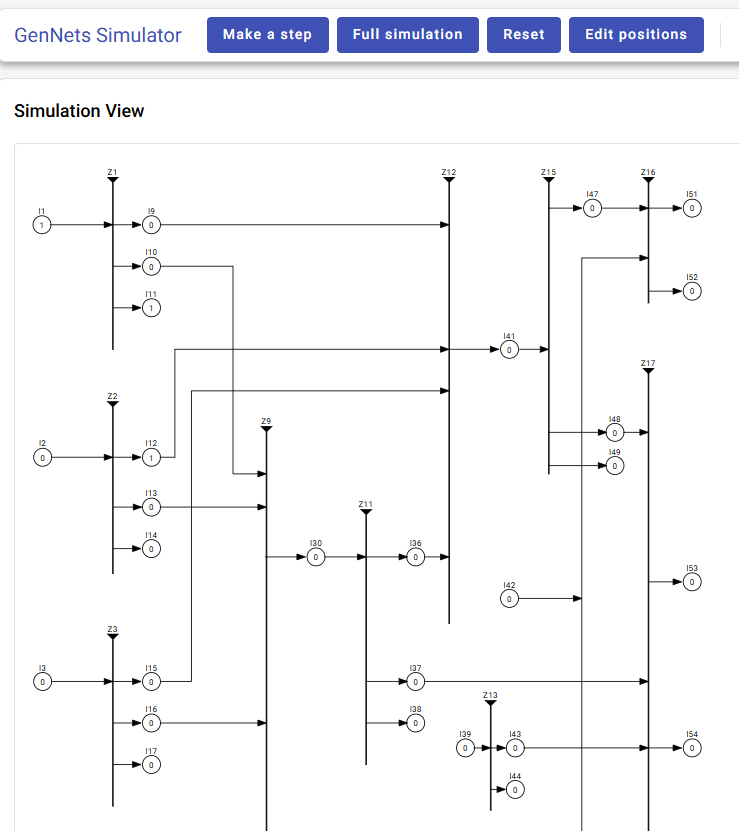
\includegraphics[width=1\linewidth]{4. applications/fuelGasEtc/images/upper.png}}
	\caption{Горна част на ОМ модела в \textit{OnlineGN}.}
	\label{fig:onlinegn-model-upper}
\end{figure}

\begin{figure}[H]
	\centering
	\setlength{\fboxrule}{2pt}
	\setlength{\fboxsep}{0pt}
	\fbox{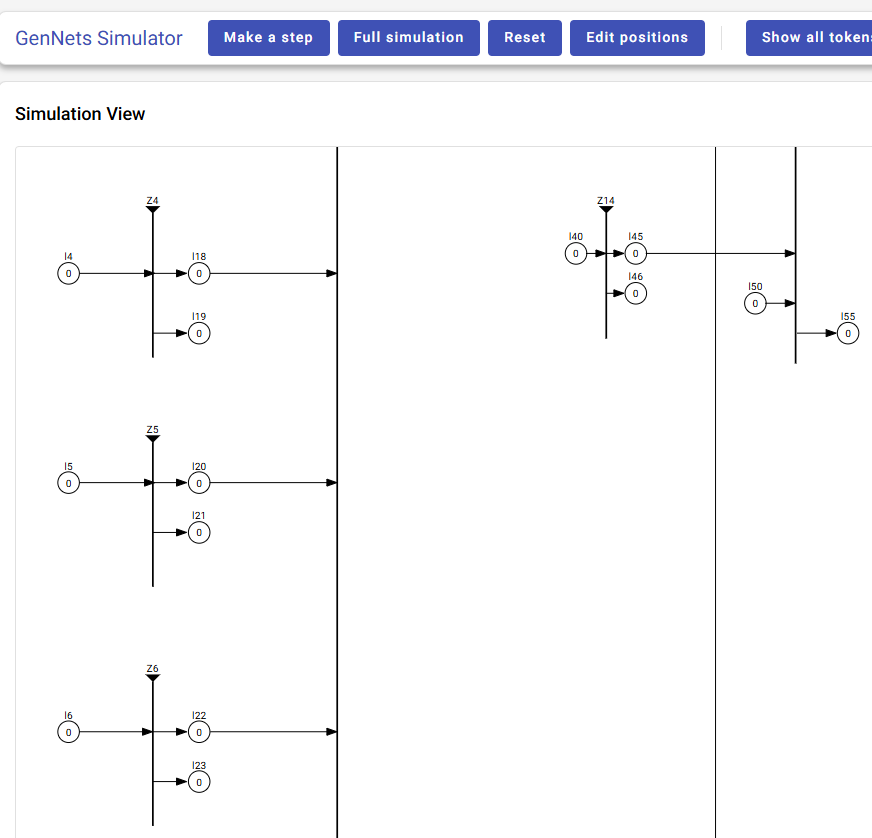
\includegraphics[width=1\linewidth]{4. applications/fuelGasEtc/images/middle.png}}
	\caption{Средна част на ОМ модела в \textit{OnlineGN}.}
	\label{fig:onlinegn-model-middle}
\end{figure}

\begin{figure}[H]
	\centering
	\setlength{\fboxrule}{2pt}
	\setlength{\fboxsep}{0pt}
	\fbox{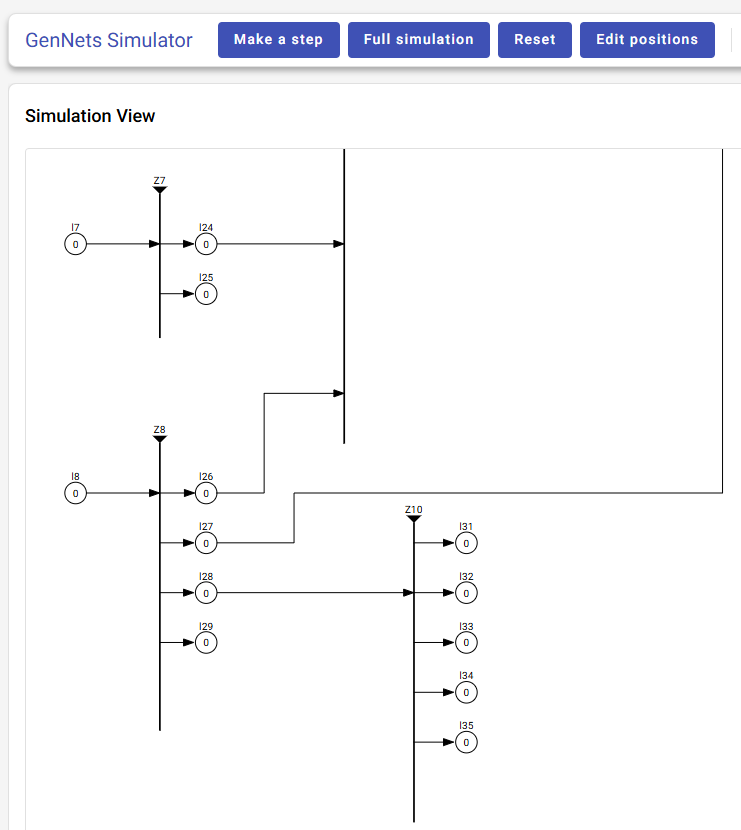
\includegraphics[width=1\linewidth]{4. applications/fuelGasEtc/images/bottom.png}}
	\caption{Долна част на ОМ модела в \textit{OnlineGN}.}
	\label{fig:onlinegn-model-lower}
\end{figure}

\vspace{0.4cm}

Следващата важна стъпка е логиката на преходите: за всеки преход са дефинирани индексирани матрици, в които са заложени предикатите от теоретичното описание. Именно тези предикати „решават“ дали дадено ядро може да премине от входните към изходните позиции на прехода. На \textbf{Фигура~\ref{fig:onlinegn-matrix-z1}} е показан пример с индексирана матрица за преход $Z_1$, който в модела съответства на \textit{CDU-2}.

\begin{figure}[H]
	\centering
	\setlength{\fboxrule}{2pt}
	\setlength{\fboxsep}{0pt}
	\fbox{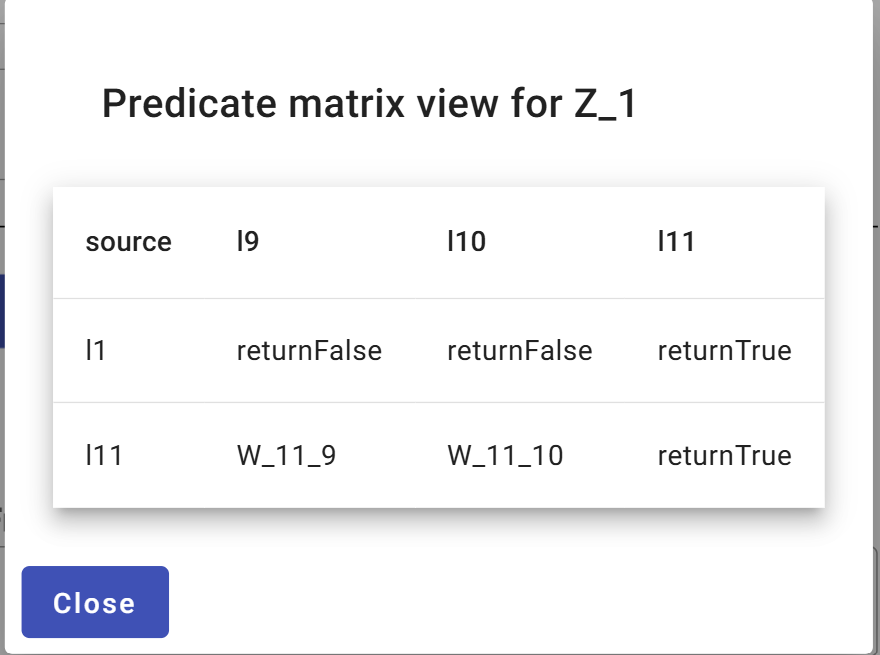
\includegraphics[width=0.5\linewidth]{4. applications/fuelGasEtc/images/matrix_1.png}}
	\captionsetup{width=0.8\textwidth}
	\caption{Индексирана матрица с предикатите за преход $Z_1$ (\textit{CDU-2}).}
	\label{fig:onlinegn-matrix-z1}
\end{figure}

В този конкретен пример предикатите отразяват условия от типа „има заявка за продукт ВПГ от \textit{CDU-2}“ и „има заявка за продукт горивен газ от \textit{CDU-2}“. С други думи, преходът $Z_1$ пропуска ядра нататък само когато са налице съответните заявки/условия, описани в модела.

Началните характеристики на ядрата са настроени според сценария от статията. На \textbf{Фигура~\ref{fig:onlinegn-token-l1}} е показано ядро във входната позиция $l_1$, което постъпва към $Z_1$ (\textit{CDU-2}), заедно с неговата начална характеристика. Тази характеристика съдържа необходимите атрибути за симулацията (например вид заявка и количества), така че по време на изпълнение да може ясно да се проследи какво „носи“ ядрото и какво се променя по веригата.

\begin{figure}[H]
	\centering
	\setlength{\fboxrule}{2pt}
	\setlength{\fboxsep}{0pt}
	\fbox{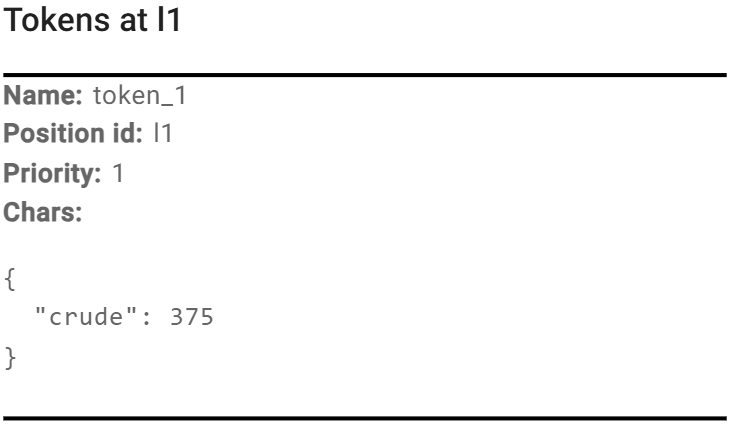
\includegraphics[width=0.5\linewidth]{4. applications/fuelGasEtc/images/token_1.png}}
	\captionsetup{width=0.8\textwidth}
	\caption{Ядро във входната позиция $l_1$ с начална характеристика (пример за вход към $Z_1$).}
	\label{fig:onlinegn-token-l1}
\end{figure}

След успешното изпълнение на симулацията наблюдаваните изходни характеристики съвпадат с очакваните теоретични резултати. Като конкретна илюстрация, на изходната позиция $l_{53}$ (обозначена като \textit{„LPG TANKS“}) се получава ядро, чиято характеристика съдържа количеството ВПГ, което моделът предвижда. Това е показано на \textbf{Фигура~\ref{fig:onlinegn-token-l53}}.

\begin{figure}[H]
	\centering
	\setlength{\fboxrule}{2pt}
	\setlength{\fboxsep}{0pt}
	\fbox{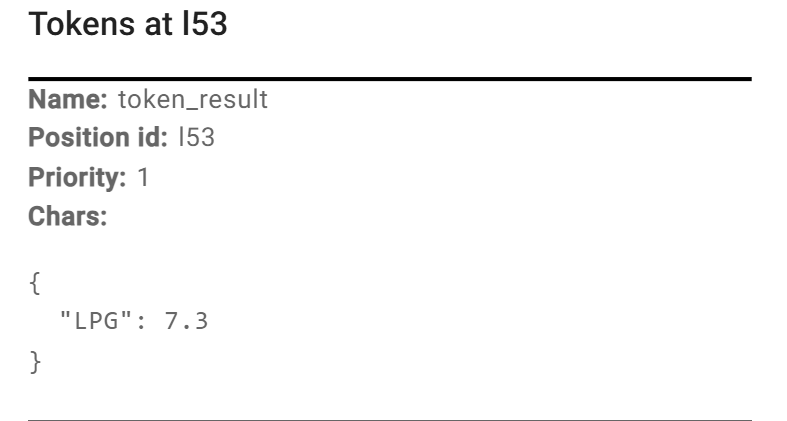
\includegraphics[width=0.5\linewidth]{4. applications/fuelGasEtc/images/token_2.png}}
	\captionsetup{width=0.8\textwidth}
	\caption{Ядро в изходната позиция $l_{53}$ (\textit{„LPG TANKS“}) с характеристика след симулация.}
	\label{fig:onlinegn-token-l53}
\end{figure}

Обобщено, симулационните резултати потвърждават, че зададените предикати и начални характеристики работят коректно и че ОМ моделът описва адекватно разглеждания производствен процес. Това дава основание да приемем модела за валидиран спрямо теоретичния сценарий и използваем за последващи експерименти и анализи.


\subsubsection{Изводи за модела и симулацията}

\hspace*{2.5em}Процесът на производство на газообразни продукти в нефтопреработвателна рафинерия -- като газово гориво, пропан-бутан (Втечнен петролен газ, ВПГ) и пропилен, които могат да се експортират като готов краен продукт или да се използват като суровина за производство на полипропилен -- представлява сложен паралелен процес, чието описание чрез линейно, а често и чрез динамично програмиране е затруднено. Основната трудност е свързана с коректното отразяване на логиката на причинно--следствените връзки, която в ОМ се задава естествено чрез предикатите на преходните условия.

Настоящата глава представя ОМ модел за производството на газово гориво, ВПГ, пропилен и полипропилен в нефтопреработвателна рафинерия, както и неговата програмна реализация и симулация. Симулацията с \textit{OnlineGN} и получаването на резултати, съответстващи на очакваното поведение на процеса, потвърждават коректността на модела и демонстрират приложимостта на ОМ при моделиране и симулация на подобни производствени вериги.


\subsection{Модел с обобщена мрежа на производството на тежки нефтопродукти в нефтопреработвателна рафинерия}

\paragraph{Декларация за принос (съвместна публикация).}
\mbox{}\\
Разделът обобщава и интегрира резултати от съвместната публикация~\cite{Stratiev2023_2}.
Личният принос на докторанта се състои в: (i) съвместно конструиране на ОМ по описанието на процеса;
(ii) изпълнение на пълната симулация в \textit{OnlineGN} с цел верификация на модела и обработка на получените резултати;
(iii) изготвяне на илюстративния материал (всички фигури от симулациите) и описание на симулационния ход в текста.
%here i put new page command
\newpage
Тук се разглежда ОМ модел на производството на тежки нефтопродукти в нефтопреработвателна рафинерия и неговата симулация чрез \textit{OnlineGN}.
Изграждането на модела е описано подробно в гореспоменатата публикация~\cite{Stratiev2023_2}.

\subsubsection{Увод в обобщеномрежовите модели за нефтопродукти в нефтопреработвателна рафинерия}


\hspace*{2.5em}В предходния раздел бе показано, че паралелно протичащите производствени процеси в нефтопреработвателна рафинерия могат да бъдат моделирани и симулирани посредством ОМ~\cite{Z1}. В настоящата глава фокусът се премества към частта от технологичната схема, свързана с преработката на тежките остатъчни фракции и производството на тежки нефтени продукти, която до момента не е била представена с ОМ.

Тежкият нефт представлява остатъчната нефтена фракция, която остава след атмосферна дестилация на суровия нефт~\cite{96}. Той съдържа компоненти с температура на кипене над 360~$^\circ$C и относителна плътност над 0.933 (\textit{API} < 20)~\cite{97}. В нефтопреработвателна рафинерия тази фракция се подлага на допълнителна обработка с цел извличане на допълнителни количества леки нефтени продукти и производство на тежки нефтени продукти като горивни масла, корабни горива и битум за пътни настилки~\cite{98}.

Процесите в технологичната верига за обработка на тежък нефт са обект на моделиране и симулация с цел по-добро разбиране на поведението на инсталациите и определяне на стойностите на оперативните променливи, които осигуряват оптимална работа от икономическа, енергоспестяваща и екологична гледна точка~\cite{103,104}. Например в ~\cite{103} се симулира работата на вакуумната дестилация на атмосферни остатъци чрез \textit{Chemcad 5.1} с цел намаляване на енергийното потребление, а в ~\cite{104} се моделира индустриален реактор със суспензионна фаза (\textit{SPR}) за хидрокрекинг на вакуумни остатъци, използвайки различни кинетични модели.

Посочените и сходни разработки са частични модели на отделни процеси за обработка на тежък нефт и често служат като вход към планови/оптимизационни модели на ниво рафинерия. В настоящата глава паралелният характер на технологичната верига се разглежда чрез ОМ модел, който позволява едновременно описание на структурните връзки и логиката на протичане на процесите, както и симулация при зададени сценарии.

Целта на настоящото изследване е да се анализира процесът по производство на различни видове тежко гориво и битум за пътни настилки в рамките на нефтопреработвателна рафинерия, да се моделира с помощта на ОМ и моделът да бъде симулиран чрез \textit{OnlineGN}.
\subsubsection{Схема на преработка за производство на различни видове тежко гориво и битум за пътни настилки в нефтопреработвателна рафинерия, моделирана чрез обобщени мрежи}

\hspace*{2.5em}Горивата, използвани основно като гориво за товарни кораби, са известни и като морски горива. Световното търсене на морски горива се оценява на около 640 000 тона на ден, което подчертава значението на този вид гориво за световната икономика~\cite{123}. В изследваната рафинерия (ЛУКОЙЛ Нефтохим Бургас, ЛНБ) се получават три вида гориво с различно съдържание на сяра: гориво с масово съдържание на сяра $\leq$ 0.5 \% (\textit{Fuel oil} 0.5\%~\textit{S}); гориво със съдържание на сяра $\leq$ 1.0\% (\textit{Fuel oil} 1.0\%~\textit{S}); и гориво със съдържание на сяра $\leq$ 2.5\% (\textit{Fuel oil} 2.5\%~\textit{S}), както е показано на \textbf{Фигура~\ref{fig1}}.

Спецификациите на трите вида гориво, произвеждани в рафинерията ЛНБ са представени подробно в статия  ~\cite{Stratiev2023_2}. Горивата, произведени в рафинерията ЛНБ, се предлагат на пазара в съответствие с приложимите изисквания, представени в~\cite{Stratiev2023_2}.

\begin{figure}[H]
  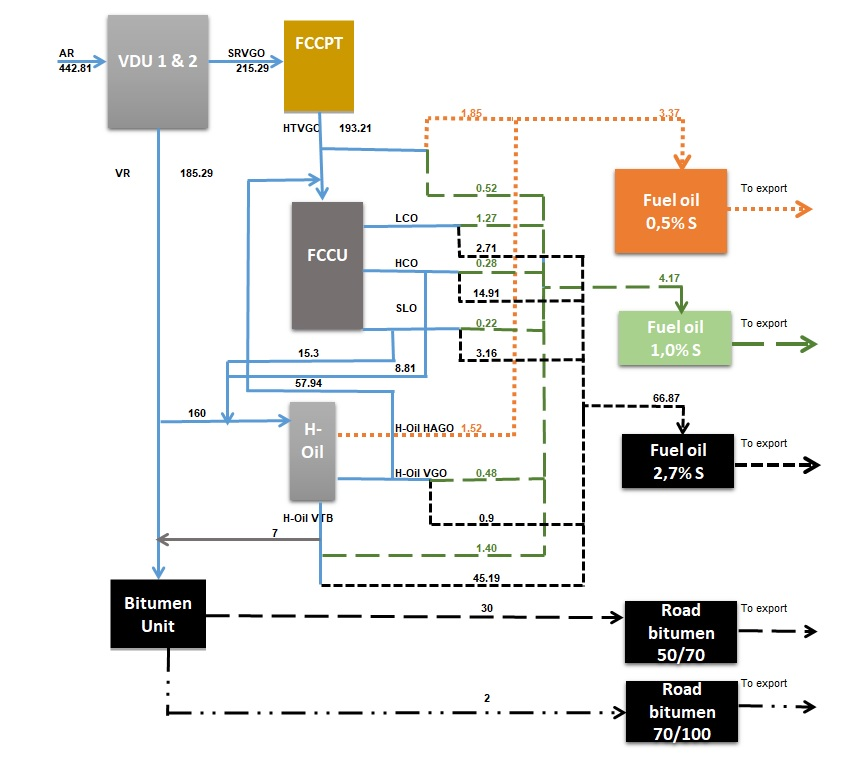
\includegraphics[scale=0.65]{4. applications/heavyOilProducts/images/Figure_1.jpg}%
  \caption{Схема на преработка
за производство на различни видове тежко гориво и битум за пътни настилки в нефтопреработвателна рафинерия, която ще бъде моделирана чрез обобщени мрежи (Числата в диаграмата съответстват на количеството потоци от тежък нефт в размер на t/h. Използвани са различни цветове за разграничаване на трите вида произведени горива: оранжев -- за гориво с 0.5\%~S, зелен -- за гориво с 1.0\%~S и черен -- за гориво с 2.5\%~S).}\label{fig1}
\end{figure}


\textbf{Фигура~\ref{fig1}} показва, че производството на битум за пътни настилки се осъществява в битумната инсталация (\textit{BU}), където смес от директен вакуумен остатък и \textit{H-Oil VTB} се подлага на окисление за получаване на два класа пътен битум: 50/70 и 70/100.

Подробности относно производството на пътен битум от директен вакуумен остатък (\textit{VR}) и \textit{H-Oil VTB} могат да се намерят в скорошно изследване~\cite{124}. Както се вижда и от \textbf{Фигура~\ref{fig1}}, вакуумният остатък (\textit{VR}) и вакуумният газьол от пряк добив (\textit{SRVGO}), използвани за производство на компонентите за горивата, както и на пътния битум, се получават в инсталациите за вакуумна дестилация (\textit{VDU-1} и \textit{VDU-2}), където атмосферният остатък, получен от инсталациите за първична дестилация на суров нефт (\textit{CDU}), се фракционира. Подробности относно работата на инсталациите за вакуумна дестилация са представени в~\cite{103}.

\subsubsection{Резултати от моделирането на производството на тежки нефтени продукти в нефтопреработвателна рафинерия с помощта на обобщени мрежи}

\hspace*{2.5em}ОМ моделът, показан на \textbf{Фигура~\ref{fig2}} съдържа 8 прехода, 35 позиции и 8 типа ядра. Значението на преходите е следното:

\begin{itemize}
	\item[$\bullet$] \textbf{\textit{VDU}} —  инсталация за вакуумна дестилация на мазута
	\item[$\bullet$] \textbf{\textit{FCCPT}} — инсталация за хидроочистване на суровината за каталитичен крекинг
	\item[$\bullet$] \textbf{\textit{H-Oil}} —  инсталация за хидрокрекинг на гудрон (\textit{H-Oil})
	\item[$\bullet$] \textbf{\textit{FCCU}} — инсталация за каталитичен крекинг на вакуумен газьол
	\item[$\bullet$] \textbf{\textit{BU}} —  инсталация за производство на пътни битуми
	\item[$\bullet$] \textbf{0.5 \textit{S}} — котелно гориво със съдържание на сяра не по-високо от 0.5~мас.\,\% \textit{S}
	\item[$\bullet$] \textbf{1.0 \textit{S}} — котелно гориво със съдържание на сяра не по-високо от 1.0~мас.\,\% \textit{S}
	\item[$\bullet$] \textbf{2.5 \textit{S}} — котелно гориво, съдържащо максимум 2.5~мас.\,\% \textit{S}
\end{itemize}



В началния момент от функционирането на ОМ ядрото $\alpha_0$ се намира в позиция $l_1$ с начална характеристика:
$$„\mbox{Атмосферен остатък (\textit{AR}), начално количество}“;$$
ядрото $\beta_0$ се намира в позиция $l_9$ с начална характеристика:
$$„\mbox{Пряко дестилатен вакуумен газьол (\textit{SRVGO}), начално количество}“;$$
ядрото $\gamma_0$ се намира в позиция $l_{17}$ с начална характеристика:
$$„\mbox{\textls[-15]{Смес от пряко дестилатен вакуумен остатък (\textit{SRVR}), \textit{FCC HCO} и \textit{FCC SLO}, начално количество}}“;$$
ядрото $\delta_0$ се намира в позиция $l_{26}$ с начална характеристика:
$$„\mbox{Смес от вакуумни газьоли, състояща се от \textit{SRVGO} и \textit{H-Oil VGO}, начално количество}“;$$
ядрото $\epsilon_0$ се намира в позиция $l_{29}$ с начална характеристика:
$$„\mbox{Смес от \textit{SRVR} и хидрокрекиран вакуумен остатък, начално количество}“;$$
ядрото $\zeta_0$ се намира в позиция $l_{31}$ с начална характеристика:
$$„\mbox{Гориво мазут с максимално съдържание на сяра 0{,}5~мас.~\%, начално количество}“;$$
ядрото $\eta_0$ се намира в позиция $l_{33}$ с начална характеристика:
$$„\mbox{Гориво мазут с максимално съдържание на сяра 1{,}0~мас.~\%, начално количество}“;$$
ядрото $\theta_0$ се намира в позиция $l_{35}$ с начална характеристика:
$$„\mbox{Гориво мазут с максимално съдържание на сяра 2{,}5~мас.~\%, начално количество}“;$$

Във всеки следващ момент от времето, в позиция $l_1$ постъпват ядра $\alpha_1, \alpha_2, ...$ с начални характеристики:
$$„\mbox{\textit{AR}, текущо постъпващо количество}“.$$

\begin{figure}[H]
		\tiny
	\newcommand{\mytriangle}{\Large $\bigtriangledown$}
	%\begin{center}
%		\begin{center}
		\setlength{\unitlength}{8.5pt} %10pt=4mm
		\linethickness{0.4pt}
		\begin{picture}(37, 71)
			%%% Transitions
			\put(3.0,71.0){\makebox(0,0)[cc]{$VDU$}}
			\put(3.0,69.0){\makebox(0,0)[bb]{\mytriangle}}
			\put(3.0,69.0){\line(0,-1){39}}
			\put(34.0,71){\makebox(0,0)[cc]{$BU$}}
			\put(34.0,69.0){\makebox(0,0)[bb]{\mytriangle}}
			\put(34.0,69.0){\line(0,-1){7}}
			\put(20.0,65.0){\makebox(0,0)[cc]{$H-Oil$}}
			\put(20.0,63.0){\makebox(0,0)[bb]{\mytriangle}}
			\put(20.0,63.0){\line(0,-1){17}}
			\put(34.0,57){\makebox(0,0)[cc]{$0.5\% S$}}
			\put(34.0,55.0){\makebox(0,0)[bb]{\mytriangle}}
			\put(34.0,55.0){\line(0,-1){7}}
			\put(20.0,39.0){\makebox(0,0)[cc]{$FCCU$}}
			\put(20.0,37.0){\makebox(0,0)[bb]{\mytriangle}}
			\put(20.0,37.0){\line(0,-1){19}}
			\put(34.0,39.0){\makebox(0,0)[cc]{$1.0\% S$}}
			\put(34.0,37.0){\makebox(0,0)[bb]{\mytriangle}}
			\put(34.0,37.0){\line(0,-1){15}}
			\put(10.0,37.0){\makebox(0,0)[cc]{$FCCPT$}}
			\put(10.0,35.0){\makebox(0,0)[bb]{\mytriangle}}
			\put(10.0,35.0){\line(0,-1){11}}
			\put(34.0,17.0){\makebox(0,0)[cc]{$2.5\% S$}}
			\put(34.0,15.0){\makebox(0,0)[bb]{\mytriangle}}
			\put(34.0,15.0){\line(0,-1){13}}
			%%% Input places
			\put(1.5,68.5){\makebox(0,0)[cc]{$l_{1}$}}
			\put(1.5,67.5){\circle{1.0}}
			\put(2.0,67.5){\vector(1,0){1.0}}
			%%% Output places
			\put(4.5,68.5){\makebox(0,0)[cc]{$l_{2}$}}
			\put(3.0,67.5){\vector(1,0){1.0}}
			\put(4.5,67.5){\circle{1.0}}
			\put(35.5,68.5){\makebox(0,0)[cc]{$l_{27}$}}
			\put(34.0,67.5){\vector(1,0){1.0}}
			\put(35.5,67.5){\circle{1.0}}
			\put(35.5,66.5){\makebox(0,0)[cc]{$l_{28}$}}
			\put(34.0,65.5){\vector(1,0){1.0}}
			\put(35.5,65.5){\circle{1.0}}
			\put(35.5,64.5){\makebox(0,0)[cc]{$l_{29}$}}
			\put(34.0,63.5){\vector(1,0){1.0}}
			\put(35.5,63.5){\circle{1.0}}
			\put(4.5,62.5){\makebox(0,0)[cc]{$l_{3}$}}
			\put(3.0,61.5){\vector(1,0){1.0}}
			\put(4.5,61.5){\circle{1.0}}
			\put(21.5,62.5){\makebox(0,0)[cc]{$l_{10}$}}
			\put(20.0,61.5){\vector(1,0){1.0}}
			\put(21.5,61.5){\circle{1.0}}
			\put(21.5,60.5){\makebox(0,0)[cc]{$l_{11}$}}
			\put(20.0,59.5){\vector(1,0){1.0}}
			\put(21.5,59.5){\circle{1.0}}
			\put(21.5,58.5){\makebox(0,0)[cc]{$l_{12}$}}
			\put(20.0,57.5){\vector(1,0){1.0}}
			\put(21.5,57.5){\circle{1.0}}
			\put(21.5,56.5){\makebox(0,0)[cc]{$l_{13}$}}
			\put(20.0,55.5){\vector(1,0){1.0}}
			\put(21.5,55.5){\circle{1.0}}
			\put(21.5,54.5){\makebox(0,0)[cc]{$l_{14}$}}
			\put(20.0,53.5){\vector(1,0){1.0}}
			\put(21.5,53.5){\circle{1.0}}
			\put(35.5,54.5){\makebox(0,0)[cc]{$l_{30}$}}
			\put(34.0,53.5){\vector(1,0){1.0}}
			\put(35.5,53.5){\circle{1.0}}
			\put(21.5,52.5){\makebox(0,0)[cc]{$l_{15}$}}
			\put(20.0,51.5){\vector(1,0){1.0}}
			\put(21.5,51.5){\circle{1.0}}
			\put(21.5,50.5){\makebox(0,0)[cc]{$l_{16}$}}
			\put(20.0,49.5){\vector(1,0){1.0}}
			\put(21.5,49.5){\circle{1.0}}
			\put(35.5,50.5){\makebox(0,0)[cc]{$l_{31}$}}
			\put(34.0,49.5){\vector(1,0){1.0}}
			\put(35.5,49.5){\circle{1.0}}
			\put(21.5,48.5){\makebox(0,0)[cc]{$l_{17}$}}
			\put(20.0,47.5){\vector(1,0){1.0}}
			\put(21.5,47.5){\circle{1.0}}
			\put(21.5,36.5){\makebox(0,0)[cc]{$l_{18}$}}
			\put(20.0,35.5){\vector(1,0){1.0}}
			\put(21.5,35.5){\circle{1.0}}
			\put(4.5,34.5){\makebox(0,0)[cc]{$l_{4}$}}
			\put(3.0,33.5){\vector(1,0){1.0}}
			\put(4.5,33.5){\circle{1.0}}
			\put(11.5,34.5){\makebox(0,0)[cc]{$l_{6}$}}
			\put(10.0,33.5){\vector(1,0){1.0}}
			\put(11.5,33.5){\circle{1.0}}
			\put(21.5,34.5){\makebox(0,0)[cc]{$l_{19}$}}
			\put(20.0,33.5){\vector(1,0){1.0}}
			\put(21.5,33.5){\circle{1.0}}
			\put(4.5,32.5){\makebox(0,0)[cc]{$l_{5}$}}
			\put(3.0,31.5){\vector(1,0){1.0}}
			\put(4.5,31.5){\circle{1.0}}
			\put(21.5,32.5){\makebox(0,0)[cc]{$l_{20}$}}
			\put(20.0,31.5){\vector(1,0){1.0}}
			\put(21.5,31.5){\circle{1.0}}
			\put(35.5,32.5){\makebox(0,0)[cc]{$l_{32}$}}
			\put(34.0,31.5){\vector(1,0){1.0}}
			\put(35.5,31.5){\circle{1.0}}
			\put(11.5,30.5){\makebox(0,0)[cc]{$l_{7}$}}
			\put(10.0,29.5){\vector(1,0){1.0}}
			\put(11.5,29.5){\circle{1.0}}
			\put(21.5,30.5){\makebox(0,0)[cc]{$l_{21}$}}
			\put(20.0,29.5){\vector(1,0){1.0}}
			\put(21.5,29.5){\circle{1.0}}
			\put(11.5,28.5){\makebox(0,0)[cc]{$l_{8}$}}
			\put(10.0,27.5){\vector(1,0){1.0}}
			\put(11.5,27.5){\circle{1.0}}
			\put(21.5,28.5){\makebox(0,0)[cc]{$l_{22}$}}
			\put(20.0,27.5){\vector(1,0){1.0}}
			\put(21.5,27.5){\circle{1.0}}
			\put(11.5,26.5){\makebox(0,0)[cc]{$l_{9}$}}
			\put(10.0,25.5){\vector(1,0){1.0}}
			\put(11.5,25.5){\circle{1.0}}
			\put(21.5,26.5){\makebox(0,0)[cc]{$l_{23}$}}
			\put(20.0,25.5){\vector(1,0){1.0}}
			\put(21.5,25.5){\circle{1.0}}
			\put(21.5,24.5){\makebox(0,0)[cc]{$l_{24}$}}
			\put(20.0,23.5){\vector(1,0){1.0}}
			\put(21.5,23.5){\circle{1.0}}
			\put(35.5,24.5){\makebox(0,0)[cc]{$l_{33}$}}
			\put(34.0,23.5){\vector(1,0){1.0}}
			\put(35.5,23.5){\circle{1.0}}
			\put(21.5,22.5){\makebox(0,0)[cc]{$l_{25}$}}
			\put(20.0,21.5){\vector(1,0){1.0}}
			\put(21.5,21.5){\circle{1.0}}
			\put(21.5,20.5){\makebox(0,0)[cc]{$l_{26}$}}
			\put(20.0,19.5){\vector(1,0){1.0}}
			\put(21.5,19.5){\circle{1.0}}
			\put(35.5,10.5){\makebox(0,0)[cc]{$l_{34}$}}
			\put(34.0,9.5){\vector(1,0){1.0}}
			\put(35.5,9.5){\circle{1.0}}
			\put(35.5,4.5){\makebox(0,0)[cc]{$l_{35}$}}
			\put(34.0,3.5){\vector(1,0){1.0}}
			\put(35.5,3.5){\circle{1.0}}
			%%% Vertical paths
			\put(30.5,65.5){\line(0,-1){4}}
			\put(31.5,63.5){\line(0,-1){3}}
			\put(36.5,63.5){\line(0,-1){3}}
			\put(31.5,59.5){\line(0,-1){6}}
			\put(30.5,57.5){\line(0,-1){22}}
			\put(29.5,55.5){\line(0,-1){22}}
			\put(26.5,53.5){\line(0,-1){40}}
			\put(15.5,51.5){\line(0,-1){8}}
			\put(25.5,51.5){\line(0,-1){40}}
			\put(28.5,51.5){\line(0,-1){10}}
			\put(16.5,49.5){\line(0,-1){9}}
			\put(23.5,49.5){\line(0,-1){10}}
			\put(31.5,49.5){\line(0,-1){3}}
			\put(36.5,49.5){\line(0,-1){3}}
			\put(17.5,47.5){\line(0,-1){3}}
			\put(22.5,47.5){\line(0,-1){3}}
			\put(24.5,43.5){\line(0,-1){10}}
			\put(12.5,41.5){\line(0,-1){8}}
			\put(22.5,40.5){\line(0,-1){5}}
			\put(17.5,39.5){\line(0,-1){4}}
			\put(0.5,31.5){\line(0,-1){3}}
			\put(5.5,31.5){\line(0,-1){3}}
			\put(13.5,27.5){\line(0,-1){12}}
			\put(7.5,25.5){\line(0,-1){3}}
			\put(12.5,25.5){\line(0,-1){3}}
			\put(24.5,25.5){\line(0,-1){16}}
			\put(29.5,25.5){\line(0,-1){10}}
			\put(23.5,23.5){\line(0,-1){16}}
			\put(31.5,23.5){\line(0,-1){3}}
			\put(36.5,23.5){\line(0,-1){3}}
			\put(30.5,21.5){\line(0,-1){16}}
			\put(17.5,19.5){\line(0,-1){3}}
			\put(22.5,19.5){\line(0,-1){3}}
			\put(31.5,3.5){\line(0,-1){3}}
			\put(36.5,3.5){\line(0,-1){3}}
			%%% Horizontal paths
			\put(30.5,65.5){\vector(1,0){3.5}}
			\put(31.5,63.5){\vector(1,0){2.5}}
			\put(31.5,60.5){\line(1,0){5}}
			\put(31.5,53.5){\vector(1,0){2.5}}
			\put(15.5,51.5){\vector(1,0){4.5}}
			\put(28.5,51.5){\vector(1,0){5.5}}
			\put(16.5,49.5){\vector(1,0){3.5}}
			\put(31.5,49.5){\vector(1,0){2.5}}
			\put(17.5,47.5){\vector(1,0){2.5}}
			\put(31.5,46.5){\line(1,0){5}}
			\put(17.5,44.5){\line(1,0){5}}
			\put(15.5,43.5){\line(1,0){9}}
			\put(12.5,41.5){\line(1,0){16}}
			\put(16.5,40.5){\line(1,0){6}}
			\put(17.5,39.5){\line(1,0){6}}
			\put(17.5,35.5){\vector(1,0){2.5}}
			\put(30.5,35.5){\vector(1,0){3.5}}
			\put(29.5,33.5){\vector(1,0){4.5}}
			\put(0.5,31.5){\vector(1,0){2.5}}
			\put(0.5,28.5){\line(1,0){5}}
			\put(7.5,25.5){\vector(1,0){2.5}}
			\put(29.5,25.5){\vector(1,0){4.5}}
			\put(31.5,23.5){\vector(1,0){2.5}}
			\put(7.5,22.5){\line(1,0){5}}
			\put(31.5,20.5){\line(1,0){5}}
			\put(17.5,19.5){\vector(1,0){2.5}}
			\put(17.5,16.5){\line(1,0){5}}
			\put(13.5,15.5){\line(1,0){16}}
			\put(26.5,13.5){\vector(1,0){7.5}}
			\put(25.5,11.5){\vector(1,0){8.5}}
			\put(24.5,9.5){\vector(1,0){9.5}}
			\put(23.5,7.5){\vector(1,0){10.5}}
			\put(30.5,5.5){\vector(1,0){3.5}}
			\put(31.5,3.5){\vector(1,0){2.5}}
			\put(31.5,0.5){\line(1,0){5}}
			%%% Horizontal paths from output places
			\put(5.0,67.5){\vector(1,0){29}}
			\put(5.0,61.5){\vector(1,0){15}}
			\put(22.0,61.5){\line(1,0){8.5}}
			\put(22.0,59.5){\line(1,0){9.5}}
			\put(22.0,57.5){\line(1,0){8.5}}
			\put(22.0,55.5){\line(1,0){7.5}}
			\put(22.0,53.5){\line(1,0){4.5}}
			\put(22.0,51.5){\line(1,0){3.5}}
			\put(22.0,49.5){\line(1,0){1.5}}
			\put(5.0,33.5){\vector(1,0){5}}
			\put(22.0,33.5){\line(1,0){2.5}}
			\put(22.0,31.5){\vector(1,0){12}}
			\put(12.0,29.5){\vector(1,0){8}}
			\put(22.0,29.5){\vector(1,0){12}}
			\put(12.0,27.5){\line(1,0){1.5}}
			\put(22.0,27.5){\vector(1,0){12}}
			\put(22.0,25.5){\line(1,0){2.5}}
			\put(22.0,23.5){\line(1,0){1.5}}
			\put(22.0,21.5){\line(1,0){8.5}}
			%%% Corners
			\put(36.0,63.5){\line(1,0){0.5}}
			\put(36.0,49.5){\line(1,0){0.5}}
			\put(22.0,47.5){\line(1,0){0.5}}
			\put(22.0,35.5){\line(1,0){0.5}}
			\put(12.0,33.5){\line(1,0){0.5}}
			\put(5.0,31.5){\line(1,0){0.5}}
			\put(12.0,25.5){\line(1,0){0.5}}
			\put(36.0,23.5){\line(1,0){0.5}}
			\put(22.0,19.5){\line(1,0){0.5}}
			\put(36.0,3.5){\line(1,0){0.5}}
		\end{picture}
	\caption{\textls[-15]{Модел на ОМ за производството на тежки петролни продукти в рафинерията „ЛУКОЙЛ Нефтохим Бургас".}}\label{fig2}
%	\end{center}
\end{figure}
 \normalsize

%here i put new page command
\newpage

За краткост по-долу ще означаваме тези ядра като $\alpha$ без (текущите) долни индекси. По същия начин ще пропускаме долните индекси на $\beta$-, $\gamma$- и $\delta$-ядрата, чийто смисъл ще бъде описан по-нататък.

Преходите на ОМ имат следните форми:

$$VDU = \left \langle\{l_{1}, l_{5}\}, \{l_{2}, l_{3}, l_{4}, l_{5} \},
\begin{array}{c|cccc}
	&  l_{2} & l_{3}  & l_{4}    & l_{5}   \\ \midrule
	l_{1} &false  & false & false &  true\\
	l_{5}  & W_{5,2} & W_{5,3}  & W_{5,4} &  true\\
\end{array} \right \rangle , $$
където: \vspace{2mm}\\
$W_{5,2} =$ „има заявка за \textit{AR} от \textit{BU}“,\\
$W_{5,3} =$ „има заявка за \textit{AR} от \textit{H-Oil}“,\\
$W_{5,4} =$ „има заявка за \textit{AR} от \textit{FCCPT}“.\vspace{2mm}

Когато $\alpha$-ядро постъпи в позиция $l_1$, в следващия момент то постъпва в позиция $l_5$ и се обединява с ядрото $\alpha_0$, което получава характеристиката:
$$„\mbox{\textit{AR}, текущо количество в резервоара}“.$$

В зависимост от вярностните стойности на предикатите $W_{5,2}, W_{5,3}, W_{5,4}$ ядрото $\alpha_0$ се разделя на две, три или четири ядра -- самото ядро $\alpha_0$ остава в позиция $l_5$ със споменатата характеристика, а ядрата $\alpha^1, \alpha^2$ и/или $\alpha^3$ получават съответно характеристиките:
\begin{itemize}
	\item „$q_1$ \textit{AR} за \textit{BU}“ в позиция $l_2$, където $q_1 \in [0, Q_1]$;
	\item „$q_2$ \textit{AR} за \textit{H-Oil}“ в позиция $l_3$, където $q_2 \in [0, Q_2]$;
	\item „$q_3$ \textit{AR} за \textit{FCCPT}“ в позиция $l_4$, където $q_3 \in [0, Q_3]$.
\end{itemize}

Тук и по-долу $Q_i$ е максималното количество за $i$-тия тежък нефтен компонент, участващ в производството на горивен мазут и битум за пътни настилки, където $1 \le i \le 26$.

$$FCCPT = \left \langle\{l_{4}, l_{9}\}, \{l_{6}, l_{7}, l_{8}, l_{9} \},
\begin{array}{c|cccc}
	&  l_{6} & l_{7}  & l_{8}    & l_{9}   \\ \midrule
	l_{4} &false  & false & false &  true\\
	l_{9}  & W_{9,6} & W_{9,7}  & W_{9,8} &  true\\
\end{array} \right \rangle , $$
където: \vspace{2mm}\\
$W_{9,6} = ~$„има заявка за \textit{HTVGO} за производство на горивен мазут с максимум 0.5 мас. \% \textit{S}“,\\
$W_{9,7} = ~$„има заявка за \textit{HTVGO} като суровина за \textit{FCC}-инсталация“,\\
$W_{9,8} = ~$„има заявка за \textit{HTVGO} за производство на горивен мазут с максимум 1.0 мас. \% \textit{S}“.\vspace{2mm}

Ядрото $\alpha^3$ от позиция $l_4$ постъпва в позиция $l_9$ и се обединява с ядрото $\beta_0$, което получава характеристиката:
$$„\mbox{Смес от вакуумни газьоли (\textit{SRVGO} и \textit{H-Oil VGO}), текущо количество в резервоара}“.$$

В зависимост от вярностните стойности на предикатите $W_{9,6}, W_{9,7}, W_{9,8}$ ядрото $\beta_0$ се разделя на две, три или четири ядра -- самото ядро $\beta_0$ остава в позиция $l_9$ със споменатата характеристика, а ядрата $\beta^1, \beta^2$ и/или $\beta^3$ получават съответно характеристиките:
\begin{itemize}
	\item „$q_4$ \textit{HTVGO} за горивен мазут с максимум 0.5 мас.\ \% \textit{S}“ в позиция $l_6$, където $q_4 \in [0, Q_4]$;
	\item „$q_5$ \textit{HTVGO} за \textit{FCC}-инсталация“ в позиция $l_7$, където $q_5 \in [0, Q_5]$;
	\item „$q_6$ \textit{HTVGO} за горивен мазут с максимум 1.0 мас.\ \% \textit{S}“ в позиция $l_8$, където $q_6 \in [0, Q_6]$.
\end{itemize}

$$H\!-\!Oil = \left \langle\{l_{3}, l_{17}, l_{18}, l_{19}\}, \{l_{10}, l_{11}, l_{12}, l_{13}, l_{14}, l_{15}, l_{16}, l_{17} \},\right.$$
$$\left. \begin{array}{c|cccccccc}
	&  l_{10} & l_{11}  & l_{12}    & l_{13}  &  l_{14} & l_{15}  & l_{16}    & l_{17}  \\ \midrule
	l_{3} &false  & false & false & false  & false & false & false & true\\
	l_{17}   & W_{17,10} & W_{17,11}  & W_{17,12} & W_{17,13} & W_{17,14} & W_{17,15}  & W_{17,16} &  true\\
	l_{18} &false  & false & false &false  & false & false & false & true\\
	l_{19} &false  & false & false & false  & false & false & false & true\\
\end{array} \right \rangle , $$
където: \vspace{2mm}\\
$W_{17,10} = $„има заявка за \textit{VTB} за битум”,\\
$W_{17,11} = $„има заявка за \textit{HAGO} за горивен мазут 0.5 мас.\% \textit{S}”,\\
$W_{17,12} = $„има заявка за \textit{VGO} за горивен мазут 1.0 мас. \% \textit{S}”,\\
$W_{17,13} = $„има заявка за \textit{VTB} за горивен мазут 1.0 мас. \% \textit{S}”,\\
$W_{17,14} = $„има заявка за \textit{VTB} за горивен мазут 2.5 мас. \% \textit{S}”,\\
$W_{17,15} = $„има заявка за \textit{VGO} за горивен мазут 2.5 мас.\% \textit{S}”,\\
$W_{17,16} = $„има заявка за \textit{VGO} като суровина за \textit{FCC}-инсталация”.\vspace{2mm}

Ядрото $\alpha^2$ от позиция $l_3$ постъпва в позиция $l_{17}$ и се обединява с ядрото $\gamma_0$, което получава характеристиката:
$$„\mbox{\textit{SRVR}, текущо количество в резервоара}“.$$

Според истинностните стойности на предикатите $W_{17,10}, \ldots, W_{17,16}$ ядрото $\gamma_0$ се разделя на две, три, …, или седем ядра – самото ядро $\gamma_0$ остава в позиция $l_{17}$ със споменатата характеристика, а ядрата $\gamma^1, …, \gamma^7$ получават съответно характеристиките:
\begin{itemize}
	\item „$q_7$ \textit{VTB} за \textit{BU}“ в позиция $l_{10}$, където $q_7 \in [0, Q_7]$;
	\item „$q_8$ \textit{HAGO} за горивен мазут 0.5 мас.\ \% \textit{S}“ в позиция $l_{11}$, където $q_8 \in [0, Q_8]$;
	\item „$q_9$ \textit{VGO} за горивен мазут 1.0 мас.\ \% \textit{S}“ в позиция $l_{12}$, където $q_9 \in [0, Q_9]$;
	\item „$q_{10}$ \textit{VTB} за горивен мазут 1.0 мас.\ \% \textit{S}“ в позиция $l_{13}$, където $q_{10} \in [0, Q_{10}]$;
	\item „$q_{11}$ \textit{VTB} за горивен мазут 2.5 мас.\ \% \textit{S}“ в позиция $l_{14}$, където $q_{11} \in [0, Q_{11}]$;
	\item „$q_{12}$ \textit{VGO} за горивен мазут 2.5 мас.\ \% \textit{S}“ в позиция $l_{15}$, където $q_{12} \in [0, Q_{12}]$;
	\item „$q_{13}$ \textit{VGO} като суровина за \textit{FCC}-инсталация“ в позиция $l_{16}$, където $q_{13} \in [0, Q_{13}]$.
\end{itemize}

$$FCCU = \left \langle\{l_{7}, l_{16}, l_{26}\}, \{l_{18}, l_{19}, l_{20}, l_{21}, l_{22}, l_{23}, l_{24}, l_{25}, l_{26} \},\right.$$
$$\left. \begin{array}{c|ccccccccc}
	&  l_{18} & l_{19}  & l_{20}    & l_{21}  &  l_{22} & l_{23}  & l_{24}      & l_{25}  & l_{26}  \\ \midrule
	l_{7}&false  &false  & false & false & false  & false & false & false & true\\
	l_{16}&false  &false  & false & false &false  & false & false & false & true\\
	l_{26}   & W_{26,18} & W_{26,19}  & W_{26,20} & W_{26,21} & W_{26,22} & W_{26,23}  & W_{26,24} & W_{26,25} &  true\\
\end{array} \right \rangle , $$
където: \vspace{2mm}\\
$W_{26,18} = $„има заявка за \textit{SLO} като суровина за \textit{H-Oil}“,\\
$W_{26,19} = $„има заявка за \textit{HCO} като суровина за \textit{H-Oil}“,\\
$W_{26,20} = $„има заявка за \textit{LCO} за горивен мазут 1.0 мас. \% \textit{S}“,\\
$W_{26,21} = $„има заявка за \textit{HCO} за горивен мазут 1.0 мас. \% \textit{S}“,\\
$W_{26,22} = $„има заявка за \textit{SLO} за горивен мазут 1.0 мас. \% \textit{S}“,\\
$W_{26,23} = $„има заявка за \textit{LCO} за горивен мазут 2.5 мас. \% \textit{S}“,\\
$W_{26,24} = $„има заявка за \textit{HCO} за горивен мазут 2.5 мас. \% \textit{S}“,\\
$W_{26,25} = $„има заявка за \textit{SLO} за горивен мазут 2.5 мас. \% \textit{S}“.\vspace{2mm}

Ядрото $\alpha$ от позиция $l_9$ и $\gamma$-ядрото от $l_{16}$ постъпват в позиция $l_{26}$ и се обединяват с ядрото $\delta_0$, което получава характеристиката:
$$„\mbox{\textit{FCC} суровина (смес от вакуумни газьоли), текущо количество в резервоара}“.$$

Според вярностните стойности на предикатите $W_{26,18}, \ldots, W_{26,25}$ ядрото $\delta_0$ се разделя на две, три, …, или осем ядра – самото ядро $\delta_0$ остава в позиция $l_{26}$ със споменатата характеристика, а ядрата $\delta^1, …, \delta^8$ получават съответно характеристиките:
\begin{itemize}
	\item „$q_{14}$ \textit{SLO} като суровина за \textit{H-Oil}“ в позиция $l_{18}$, където $q_{14} \in [0, Q_{14}]$;
	\item „$q_{15}$ \textit{HCO} като суровина за \textit{H-Oil}“ в позиция $l_{19}$, където $q_{15} \in [0, Q_{15}]$;
	\item „$q_{16}$ \textit{LCO} за горивен мазут 1.0 мас.\ \% \textit{S}“ в позиция $l_{20}$, където $q_{16} \in [0, Q_{16}]$;
	\item „$q_{17}$ \textit{HCO} за горивен мазут 1.0 мас.\ \% \textit{S}“ в позиция $l_{21}$, където $q_{17} \in [0, Q_{17}]$;
	\item „$q_{18}$ \textit{SLO} за горивен мазут 1.0 мас.\ \% \textit{S}“ в позиция $l_{22}$, където $q_{18} \in [0, Q_{18}]$;
	\item „$q_{19}$ \textit{LCO} за горивен мазут 2.5 мас.\ \% \textit{S}“ в позиция $l_{23}$, където $q_{19} \in [0, Q_{19}]$;
	\item „$q_{20}$ \textit{HCO} за горивен мазут 2.5 мас.\ \% \textit{S}“ в позиция $l_{24}$, където $q_{20} \in [0, Q_{20}]$;
	\item „$q_{21}$ \textit{SLO} за горивен мазут 2.5 мас.\ \% \textit{S}“ в позиция $l_{25}$, където $q_{21} \in [0, Q_{21}]$.
\end{itemize}

$$BU = \left \langle\{l_{2}, l_{10}, l_{29}\}, \{l_{27}, l_{28}, l_{29} \},
\begin{array}{c|ccc}
	& l_{27}  & l_{28}    & l_{29}   \\ \midrule
	l_{2} &false  & false &  true\\
	l_{10} &false  & false &  true\\
	l_{29}  & W_{29,27} & W_{29,28}  &  true\\
\end{array} \right \rangle , $$
където: \vspace{2mm}\\
$W_{29,27} = $„има заявка за пътен битум клас 50/70“,\\
$W_{29,28} = $„има заявка за пътен битум клас 70/100“.\vspace{2mm}

Ядрото $\alpha$ от позиция $l_2$ и ядрото $\gamma$ от $l_{10}$ постъпват в позиция $l_{29}$ и се обединяват с ядрото $\epsilon_0$, което получава характеристиката:
$$„\mbox{Битумна суровина (смес от \textit{SRVR} и \textit{H-Oil VTB}), текущо количество в резервоара}“.$$

В зависимост от вярностните стойности на предикатите $W_{29,27}$ и $W_{29,28}$ ядрото $\epsilon_0$ се разделя на две или три ядра -- самото ядро $\epsilon_0$ остава в позиция $l_{29}$ със споменатата характеристика, а ядрата $\epsilon^1$ и $\epsilon^2$ получават съответно характеристиките:
\begin{itemize}
	\item „$q_{22}$ пътен битум клас 50/70“ в позиция $l_{27}$, където $q_{22} \in [0, Q_{22}]$;
	\item „$q_{23}$ пътен битум клас 70/100“ в позиция $l_{28}$, където $q_{23} \in [0, Q_{23}]$.
\end{itemize}

$$0.5\%\,S = \left \langle\{l_{6}, l_{11}, l_{31}\}, \{l_{30}, l_{31} \},
\begin{array}{c|cc}
	& l_{30}  & l_{31}    \\ \midrule
	l_{6} &false  &  true\\
	l_{11} &false &  true\\
	l_{31}  & W_{31,30} &  true\\
\end{array} \right \rangle , $$
където:\\
$W_{31,30} = $„има заявка за горивен мазут с максимум 0.5 мас.\% \textit{S}“.\vspace{2mm}

Ядрото $\gamma$ от позиция $l_{11}$ и ядрото $\beta$ от $l_7$ постъпват в позиция $l_{31}$ и се обединяват с ядрото $\zeta_0$, което получава характеристиката:
$$„\mbox{Горивен мазут с максимум 0.5 мас. \% \textit{S}, текущо количество в резервоара}“.$$

Когато предикатът $W_{31,30}$ е $true$, ядрото $\zeta_0$ се разделя на две ядра -- самото $\zeta_0$ остава в позиция $l_{31}$ със споменатата характеристика, а ядрото $\zeta^1$ получава характеристиката:
$$„\mbox{$q_{24}$ заявено количество горивен мазут с максимум 0.5 мас. \% \textit{S}}“$$
в позиция $l_{30}$, където $q_{24} \in [0, Q_{24}]$.

$$1.0\%\,S = \left \langle\{l_ {8}, l_{12}, l_{13}, l_{20}, l_{21}, l_{22}, l_{33}\}, \{l_{32}, l_{33} \},
\begin{array}{c|cc}
	& l_{32}  & l_{33}    \\ \midrule
        l_{8}  &false  &  true \\
	l_{12} &false  &  true\\
	l_{13} &false &  true\\
	l_{20} &false &  true\\
	l_{21} &false &  true\\
	l_{22} &false &  true\\
	l_{33}  & W_{33,32} &  true\\
\end{array} \right \rangle , $$
\newpage
където:\vspace{2mm}\\
$W_{33,32} = $„има заявка за горивен мазут с максимум 1.0 мас.\% \textit{S}“.\vspace{2mm}

Ядрата $\gamma$ от позиции $l_{12}$ и $l_{13}$ и ядрата $\delta$ от позиции $l_{20}, l_{21}, l_{22}$ постъпват в позиция $l_{33}$ и се обединяват с ядрото $\eta_0$, което получава характеристиката:
$$„\mbox{Горивен мазут с максимум 1.0 мас. \% \textit{S}, текущо количество в резервоара}“.$$

Когато предикатът $W_{33,32}$ е $true$, ядрото $\eta_0$ се разделя на две ядра -- самото $\eta_0$ остава в позиция $l_{33}$ със споменатата характеристика, а ядрото $\eta^1$ получава характеристиката:
$$„\mbox{$q_{25}$ заявено количество горивен мазут с максимум 1.0 мас. \% \textit{S}}“$$
в позиция $l_{32}$, където $q_{25} \in [0, Q_{25}]$.

$$2.5\%\,S = \left \langle\{l_{14}, l_{15}, l_{23}, l_{24}, l_{25}, l_{35}\}, \{l_{34}, l_{35} \},
\begin{array}{c|cc}
	& l_{34}  & l_{35}    \\ \midrule
	l_{14} &false  &  true\\
	l_{15} &false &  true\\
	l_{23} &false &  true\\
	l_{24} &false &  true\\
	l_{25} &false &  true\\
	l_{35}  & W_{35,34} &  true\\
\end{array} \right \rangle , $$
където: \vspace{2mm}\\
$W_{35,34} = $„има заявка за горивен мазут с максимум 2.5 мас.\% \textit{S}“.\vspace{2mm}

Ядрата $\gamma$ от позиции $l_{14}$ и $l_{15}$ и ядрата $\delta$ от позиции $l_{23}, l_{24}, l_{25}$ постъпват в позиция $l_{35}$ и се обединяват с ядрото $\theta_0$, което получава характеристиката:
$$„\mbox{Горивен мазут с максимум 2.5 мас. \% \textit{S}, текущо количество в резервоара}“.$$

Когато предикатът $W_{35,34}$ е $true$, ядрото $\theta_0$ се разделя на две ядра -- самото $\theta_0$ остава в позиция $l_{35}$ със споменатата характеристика, а ядрото $\theta^1$ получава характеристиката:
$$„\mbox{$q_{26}$ заявено количество горивен мазут с максимум 2.5 мас. \% \textit{S}}“$$
в позиция $l_{34}$, където $q_{26} \in [0, Q_{26}]$.

\vspace{0.3cm}

\subsubsection{Симулиране на модела с \textit{OnlineGN}}

\hspace*{2.5em}Този раздел представя симулация на модел на ОМ, който описва производството на тежки нефтопродукти в нефтопреработвателна рафинерия. Моделът е реализиран и изпълнен с \textit{OnlineGN}. Целта е да се проследи потокът на материалните ядра (представляващи междинни и крайни нефтени фракции) през основните технологични звена на рафинерията и да се квантифицират получените продуктови потоци.

\paragraph{Преглед на модела и симулацията.}
\mbox{}\\
ОМ обхваща основния път на преработка на тежки нефтопродукти, започващ от атмосферния остатък (\textit{AR}) и преминаващ през инсталации като вакуумна дестилация на мазута (\textit{VDU}), производство на пътни битуми (\textit{BU}), хидрокрекинг (\textit{H-Oil}) и предобработваща инсталация за хидроочистване на суровината за каталитичен крекинг (\textit{FCCPT}). За яснота, спомагателните входно--изходни позиции, които служат само като буфери за неизползвани количества, са пропуснати в графичното представяне. В това изследване се приема, че всички произведени количества се насочват към следващите по веригата звена, без натрупване на неизползвани междинни продукти.

\textbf{Фигура~\ref{fig:model}} показва схемата на ОМ, както е интегрирана в симулатора.

\begin{figure}[H]
	\centering
	\setlength{\fboxrule}{2pt}
	\setlength{\fboxsep}{0pt}
	\fbox{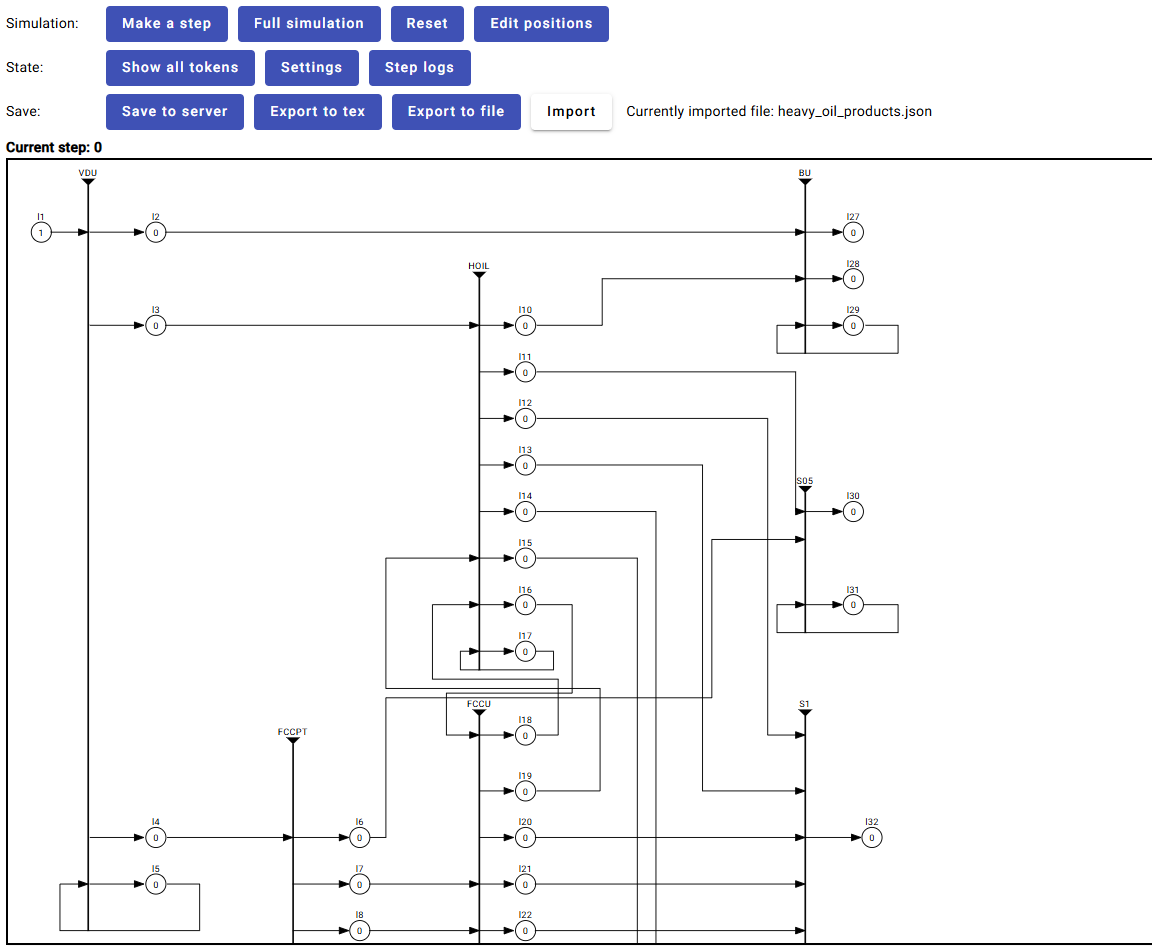
\includegraphics[width=0.95\linewidth]{4. applications/heavyOilProducts/images/model5.png}}
	\captionsetup{width=0.9\textwidth}
	\caption{Модел на обобщена мрежа (ОМ) на веригата за преработка на тежки нефтопродукти в рафинерията.}
	\label{fig:model}
\end{figure}

\paragraph{Начални условия.}
\mbox{}\\
Първоначалното ядро, разположено в позиция $l_1$, представлява атмосферен остатък с характеристична стойност 442.81 (в единици, съответстващи на оригиналния набор данни на рафинерията). Това начално условие е директно зададено в симулацията, както е показано на \textbf{Фигура~\ref{fig:init_token}}.

\begin{figure}[H]
	\centering
	\setlength{\fboxrule}{2pt}
	\setlength{\fboxsep}{0pt}
	\fbox{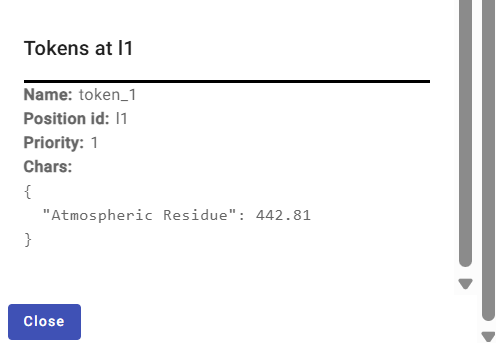
\includegraphics[width=0.6\linewidth]{4. applications/heavyOilProducts/images/init_token_char.png}}
	\captionsetup{width=0.7\textwidth}
	\caption{Инициализация на характеристиката на ядрото за атмосферния остатък в позиция $l_1$.}
	\label{fig:init_token}
\end{figure}

\paragraph{Първи етап на преработка: Вакуумна дестилация.}
\mbox{}\\
В първата моделирана стъпка ядрото за атмосферния остатък (\textit{AR}) се насочва към вакуумната дестилационна инсталация на мазута (\textit{VDU}). Поведението на \textit{VDU} се управлява от нейната индексирана матрица на прехода и съответните характеристични функции. Всяка двойка колона/ред в матрицата определя логиката за насочване на ядрото при зададени условия.

\textbf{Фигура~\ref{fig:vdu_matrix}} представя индексираната матрица за прехода в \textit{VDU}, както е конфигурирана в \textit{OnlineGN}.

\begin{figure}[H]
	\centering
	\setlength{\fboxrule}{2pt}
	\setlength{\fboxsep}{0pt}
	\fbox{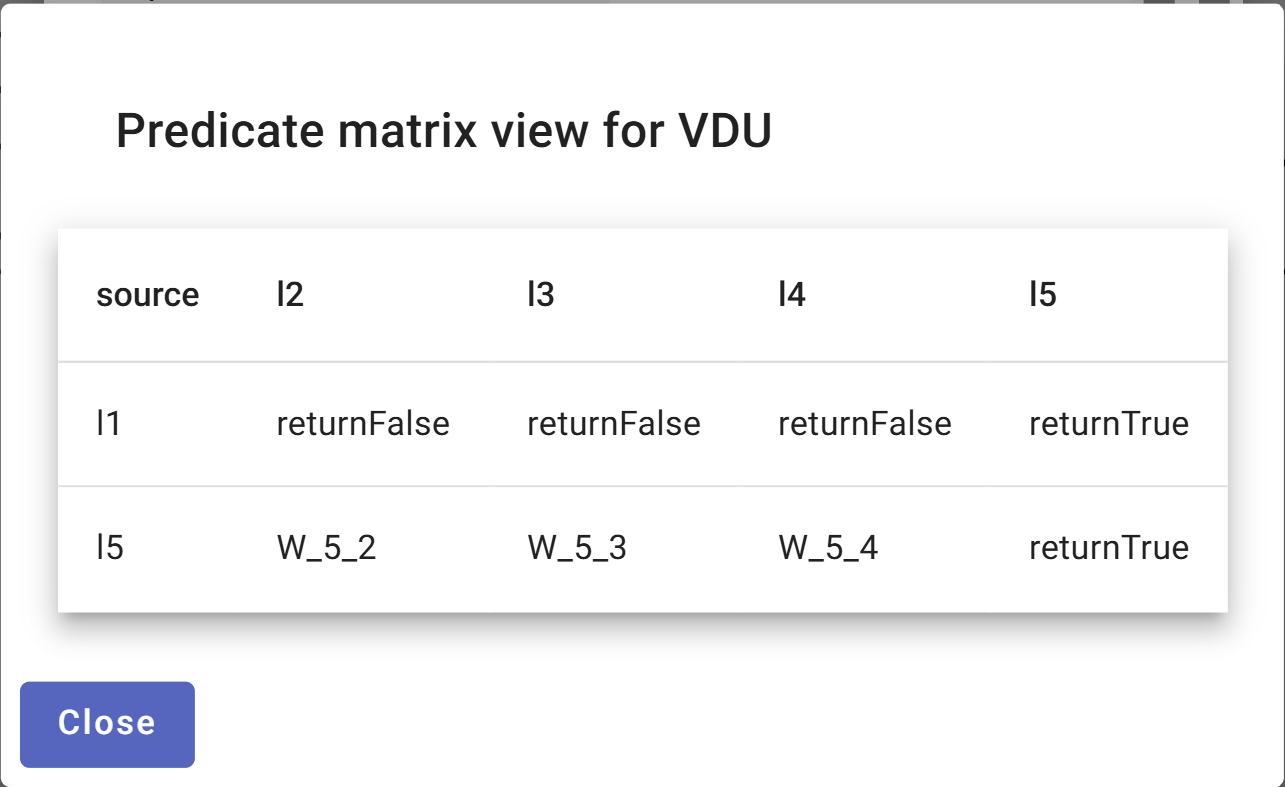
\includegraphics[width=0.6\linewidth]{4. applications/heavyOilProducts/images/matrix1.png}}
	\captionsetup{width=0.7\textwidth}
	\caption{Индексирана матрица на прехода във \textit{VDU}.}
	\label{fig:vdu_matrix}
\end{figure}

За текущия сценарий на симулация се приемат активни заявки от инсталациите \textit{BU}, \textit{H-Oil} и \textit{FCCPT}. Съответно, характеристичните функции („\textit{code}“), свързани с прехода във \textit{VDU}, са зададени както е показано на \textbf{Фигура~\ref{fig:vdu_functions}}. Тези функции могат лесно да бъдат модифицирани, за да отразят промени в потребностите на следващите звена по веригата или в оперативните ограничения.

\begin{figure}[H]
	\centering
	\setlength{\fboxrule}{2pt}
	\setlength{\fboxsep}{0pt}
	\fbox{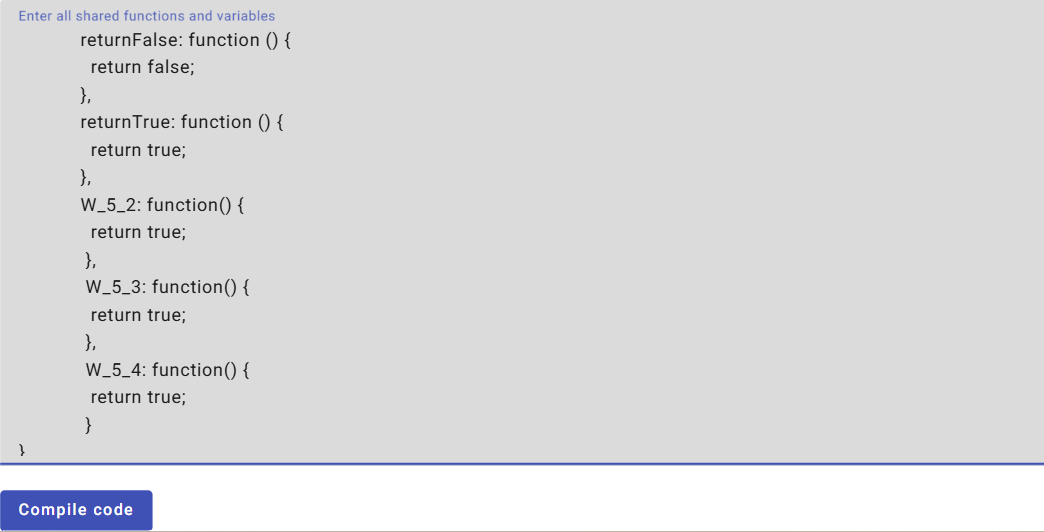
\includegraphics[width=0.8\linewidth]{4. applications/heavyOilProducts/images/functions1.png}}
	\captionsetup{width=0.8\textwidth}
	\caption{Характеристични функции, които управляват насочването на ядрото от \textit{VDU} при разглеждания сценарий за търсене.}
	\label{fig:vdu_functions}
\end{figure}

\paragraph{Следващи преработвателни инсталации.}
\mbox{}\\
Същият подход на моделиране се прилага и за останалите технологични звена. Като пример, индексираната матрица на \textit{FCCPT} е показана на \textbf{Фигура~\ref{fig:fccpt_matrix}}. Всяка матрица определя допустимите потоци и логическите условия, при които ядрата извършват преходи между позиции.

\begin{figure}[H]
	\centering
	\setlength{\fboxrule}{2pt}
	\setlength{\fboxsep}{0pt}
	\fbox{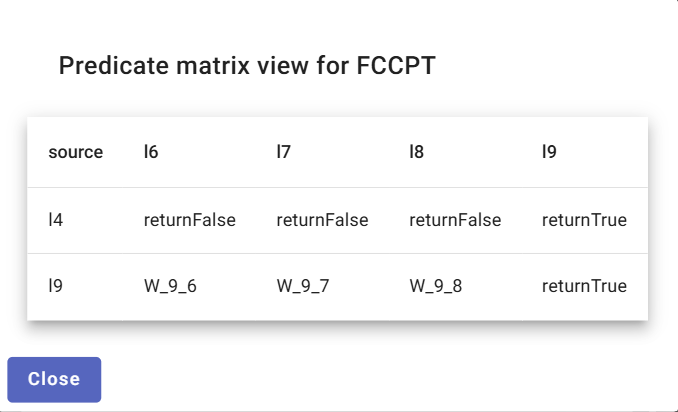
\includegraphics[width=0.6\linewidth]{4. applications/heavyOilProducts/images/matrix2.png}}
	\caption{Индексирана матрица на прехода във \textit{FCCPT}.}
	\label{fig:fccpt_matrix}
\end{figure}

\paragraph{Резултати от симулацията.}
\mbox{}\\
След изпълнение на симулацията на ОМ, количествените резултати за всеки краен продуктов поток се извеждат от характеристиките на ядрата, разположени в съответните позиции. Например количеството мазут с максимално съдържание на сяра до 1.0 мас.\% се определя от характеристичната стойност на ядрото, намиращо се в позиция \(l_{32}\) (\textbf{Фигура~\ref{fig:res1}}).

\begin{figure}[H]
	\centering
	\setlength{\fboxrule}{2pt}
	\setlength{\fboxsep}{0pt}
	\fbox{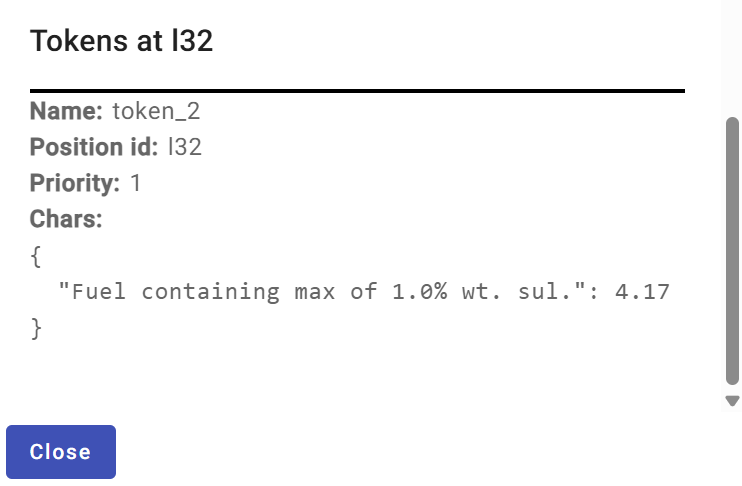
\includegraphics[width=0.6\linewidth]{4. applications/heavyOilProducts/images/1r.png}}
	\captionsetup{width=0.7\textwidth}
	\caption{Полученото количество за мазут с максимум 1.0 мас.\% сяра (позиция $l_{32}$).}
	\label{fig:res1}
\end{figure}

По аналогичен начин, количеството мазут с максимум 2.5 мас.\% сяра се представя от характеристичната стойност на ядрото в позиция $l_{34}$ (\textbf{Фигура~\ref{fig:res2}}).

\begin{figure}[H]
	\centering
	\setlength{\fboxrule}{2pt}
	\setlength{\fboxsep}{1pt}
	\fbox{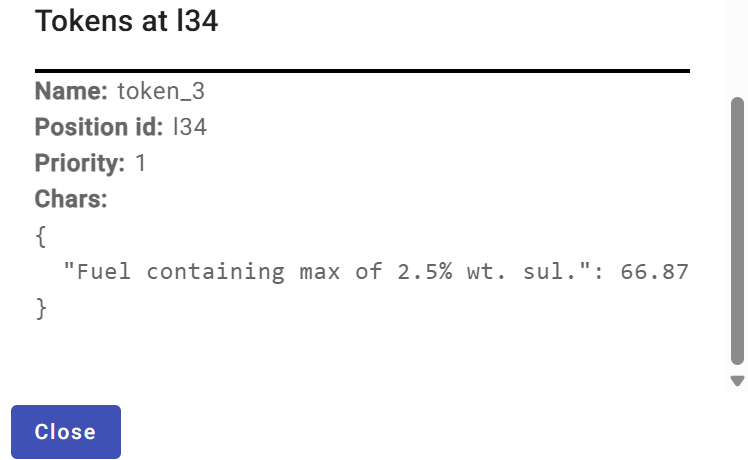
\includegraphics[width=0.6\linewidth]{4. applications/heavyOilProducts/images/2.5r.png}}
	\captionsetup{width=0.7\textwidth}
	\caption{Полученото количество за мазут с максимум 2.5 мас.\% сяра (позиция $l_{34}$).}
	\label{fig:res2}
\end{figure}

\subsubsection{Резултати за модела}

\hspace*{2.5em}Както се вижда на \textbf{Фигура~\ref{fig1}}, производството на трите класа тежко гориво (мазут) и трите класа пътен битум представлява сложен паралелен процес, който включва пет технологични инсталации (\textit{VDU}, \textit{FCCPT}, \textit{FCCU}, \textit{H-Oil} и \textit{BU}), в рамките на които се получават десет рафинирани тежки нефтени продукта. Чрез подходящо смесване на тези десет продукта, отчитащо вариациите в техните физикохимични свойства, разгледани в предходни изследвания~\cite{124}, се получават петте крайни тежки продукта. Този сложен паралелен процес може да бъде моделиран чрез използване на ОМ.

Разработеният ОМ модел за производството на различни класове тежки мазути и пътни битуми в рафинерията е четвъртият и последен модел, след предходните модели за производство на автомобилен бензин~\cite{93}, дизелово гориво~\cite{88}, както и горивен газ, втечнен петролен газ (ВПГ; \textit{LPG}), пропилен и полипропилен~\cite{Stratiev2023_1}.

Представеният модел има обобщен характер и ще бъде част (подмрежа) от бъдещ йерархичен производствен модел. Този ОМ модел от по-високо ниво ще обединява вече разработените модели за производство на отделни рафинирани продукти в едно цяло, което ще позволи цялостен анализ на работата на рафинерията и вземане на решения по отношение на влиянието на различни фактори, като прекъсвания в доставките на суровина, възникване на непланирани спирания, оптимизация на производствения процес, оценка на приложимостта на включването на нови технологични звена и др.

Обикновено линейното програмиране се използва в ситуации, при които е известно, че определено количество суровина с определени характеристики ще бъде доставено след определен период от време. Когато обаче тази яснота липсва поради динамичния характер на процесите, инструментите на линейното програмиране не са достатъчни за адекватно програмиране и планиране -- например при внезапни промени в цената на суровия нефт, в търсенето и предлагането на определени нефтени продукти и др. В рамките на ОМ модел може да се представи всичко, което се получава чрез линейно програмиране, като необходимата информация се задава чрез характеристиките на определени ядра в мрежата.

От друга страна, даден ОМ модел може да бъде включен като подмрежа в ОМ модел на експертна система, вземаща решения за определени ситуации ~\cite{GN-IFS}. Освен това в друга подмрежа могат да се симулират различни сценарии за разглеждания модел с цел проследяване как реален процес би протекъл при конкретни условия. Всеки такъв ОМ ще бъде йерархично включен в следващ модел, който се планира да бъде разработен в близко бъдеще.


\subsubsection{Изводи}

\hspace*{2.5em}Получените резултати показват, че процесите по производство на различни класове тежки нефтени продукти в рафинерия могат да бъдат успешно моделирани чрез ОМ. Подобно на разгледаните в предходната глава производствени вериги, и тук процесите са сложни и паралелни, като ОМ моделът позволява естествено представяне на причинно--следствените зависимости и технологичните ограничения.

Проведената симулация чрез \textbf{\textit{OnlineGN}} води до резултати, съответстващи на очакваното поведение на системата, което служи като верификация на коректността на модела и потвърждава приложимостта на ОМ при моделиране и симулация на производствени процеси в нефтопреработвателна рафинерия.





